\documentclass[
    a4paper,
    toc=index,
    12pt,
    DIV=14,
    twoside,
    BCOR=2cm,
    headsepline,
    numbers=noenddot,
    bibliography=totoc,
]{scrbook}

\usepackage{scrhack}
\usepackage[utf8]{inputenc}
\DeclareUnicodeCharacter{00A0}{~}   % replace non-breaking space
\usepackage[T1]{fontenc}
\usepackage[american]{babel}    % Use either American or British English consistently
\hyphenation{name-space}

\usepackage[
    n,%orlambda
    advantage,
    operators,
    sets,
    adversary,
    landau,
    probability,
    notions,
    logic,
    ff,
    mm,
    primitives,
    events,
    complexity,
    oracles,
    asymptotics,
    keys
]{cryptocode}


\definecolor{codegreen}{rgb}{0,0.6,0}
\definecolor{codegray}{rgb}{0.5,0.5,0.5}
\definecolor{codepurple}{rgb}{0.58,0,0.82}
\definecolor{backcolour}{rgb}{0.95,0.95,0.92}


\newcommand{\highlight}[1]{%
  \colorbox{yellow}{$\displaystyle#1$}
}


\newcommand{\thesisTitle}{Security Analysis of the SCION Internet Architecture}
\newcommand{\thesisType}{Master's Thesis}
\newcommand{\thesisAuthor}{Marco Georges Seewer}
\newcommand{\thesisStudentID}{19-915-776}
\newcommand{\thesisEmail}{mseewer@student.ethz.ch}
\newcommand{\thesisSupervisors}{Dr.~Roland~Meier\\Jordi~Subirà~Nieto\\Prof.~Dr.~Adrian Perrig}

\newcommand{\thesisSemester}{Spring 2024}
\newcommand{\thesisSubmission}{August 31, 2024}
\NewDocumentCommand{\img}{O{} O{} O{} O{0.75\textwidth} O{}}{
    \begin{figure}[#5]
        \centering
        \includegraphics[width=#4]{#1}
        \caption{#2}
        \label{fig:#3}
    \end{figure}
}


%
% Mathematics
\usepackage{amsmath,amsthm,amssymb,amsfonts}
\usepackage{mathtools}
%
% Fonts
\usepackage{newpxtext,newpxmath} % Palatino font, remove or change according to your taste
\usepackage{microtype} 	         % Better kerning
%
% Layout
\usepackage{multicol}   % Allows multi-column layout
\usepackage{float}      % Better interface for defining floating objects
\usepackage{flafter}    % Always place floats _after_ their definition
%
% Nicer-looking tables
\usepackage{booktabs,tabularx}
%
% Correct and consistent units and numbers
\usepackage[mode=text, math-rm=\text, detect-all, binary-units=true, per-mode=symbol, range-phrase=\,--\,, range-units=single, detect-weight=true, detect-family=true]{siunitx}
%
% Drawing and plotting
\usepackage{tikz}
\usepackage{pgfplots}
\pgfplotsset{compat=1.17}
%
% Nice and consistent quotation marks
\usepackage{csquotes}
%
% Figures
\usepackage{graphicx}
\usepackage{wrapfig}    % Wrap text around figures
\usepackage{subfig}     % Create subfigures
\graphicspath{{resources/},{figures/}}
%
% Miscellaneous
\usepackage[nice]{nicefrac} % Display ½ nicely
\usepackage{enumitem}       % Allows customizing enumerate counters
\usepackage{xcolor}         % Colors!
\usepackage{pdfpages}       % For including the declaration of originality
%
% Bibliography
\usepackage{natbib}
%
% Hyperref package for links in TOC, index, PDF metadata, bookmarks, etc.
\usepackage[plainpages=false,pdfpagelabels,bookmarks=true,backref=false,pagebackref=false]{hyperref}
\hypersetup{
    pdfauthor={\thesisAuthor},
    pdftitle={\thesisTitle},
    pdfsubject={\thesisType},
    hidelinks,
    breaklinks=true,
    pdfhighlight=/I,
    bookmarksopen=false,
    bookmarksnumbered=true
}
%
% Easy and consistent references
\usepackage[capitalize]{cleveref}
\newcommand{\crefrangeconjunction}{--}
\newcommand{\crefpairconjunction}{ and }
\newcommand{\crefmiddleconjunction}{, }
\newcommand{\creflastconjunction}{, and }
\crefname{section}{\S}{Sections}
\Crefname{section}{Section}{Sections}
\crefformat{section}{\S#2#1#3}
\Crefformat{section}{Section~#2#1#3}
\crefformat{footnote}{#2\footnotemark[#1]#3}
%
% Basic source formatting
\usepackage{listings}
% \usepackage{listings-golang} % import this package after listings
\lstloadlanguages{C, Python, Go}
\lstset{
    numbers=left,
    numberstyle=\tiny,
    numbersep=5pt,
    language=C,
    basicstyle=\ttfamily\scriptsize,
    tabsize=4,
    breaklines=true
}
%
% ETH Colors
\definecolor{eth1}{HTML}{1F407A}
\definecolor{eth2}{HTML}{3C5A0F}
\definecolor{eth3}{HTML}{0069B4}
\definecolor{eth4}{HTML}{72791C}
\definecolor{eth5}{HTML}{91056A}
\definecolor{eth6}{HTML}{6F6F6E}
\definecolor{eth7}{HTML}{A8322D}
\definecolor{eth8}{HTML}{007A92}
\definecolor{eth9}{HTML}{956013}
\definecolor{eth10}{HTML}{82BE1E}
%
%
% No single lines at the start of a paragraph ("Schusterjungen")
\clubpenalty = 10000
%
% No single lines at the end of a paragraph ("Hurenkinder")
\widowpenalty = 10000 \displaywidowpenalty = 10000
%
\renewcommand{\topfraction}{1.0}    % Figures can appear at start of page
\renewcommand{\bottomfraction}{1.0} % Figures can appear at end of page

\newcommand{\gennote}[3][blue]{\textcolor{#1}{\ $\rule{8pt}{8pt}_{\textsf{\scshape\bfseries #2}}$ #3}}
\newcommand{\ck}[1]{\gennote[violet]{CK}{#1}}


\begin{document}


\lstdefinestyle{mystyle}{
    backgroundcolor=\color{backcolour},   
    commentstyle=\color{codegreen},
    keywordstyle=\color{magenta},
    numberstyle=\tiny\color{codegray},
    stringstyle=\color{codepurple},
    basicstyle=\ttfamily\footnotesize,
    breakatwhitespace=false,         
    breaklines=true,                 
    captionpos=b,                    
    keepspaces=true,                 
    numbers=left,                    
    numbersep=5pt,                  
    showspaces=false,                
    showstringspaces=false,
    showtabs=false,                  
    tabsize=2,
    morekeywords={Element},
}

\lstset{style=mystyle}
\lstset{escapeinside={(*@}{@*)}}


\frontmatter

\begin{titlepage}

\flushleft

\vspace*{-20mm}
{
    
\includegraphics[width=5cm]{ETHlogo}
    \hfill
    
\includegraphics[width=5cm]{logo_armasuisse}
}

\vfill

{\Large \sffamily \bfseries \thesisType}\\[3mm]
Cyber Defense Campus, armasuisse Science and Technology\\
Network Security Group, Department of Computer Science, ETH Zurich

\vfill
\vfill

\begin{center}
    {\Huge \sffamily \bfseries \thesisTitle}\\[10mm]
    {\Large by \thesisAuthor}\\[8mm]
    {\large \thesisSemester}
\end{center}

\vfill
\vfill
\vfill

\renewcommand{\arraystretch}{1.1}

\begin{tabular}{b{40mm}l}
    ETH student ID:     & \thesisStudentID \\
    E-mail address:     & \thesisEmail \\\vspace*{5mm}
    Supervisors:        & \parbox[t]{10cm}{\thesisSupervisors}\\\vspace*{5mm}
    Date of submission: & \thesisSubmission
\end{tabular}

\end{titlepage}


\chapter*{Abstract}
\addcontentsline{toc}{chapter}{Abstract}

% * Briefly motivate problem domain, why is it an important domain?
% * What problem does the thesis solve?
% * What is the main contribution? -> The abstract should convince a reader to read the thesis, not necessary to explain anything, just provide an incentive to read
% * Keep the abstract short! A half page is enough.




% The increasing complexity and interconnectivity of modern networks necessitate robust security measures to protect against evolving threats.
This thesis analyzes the security of the SCION, a next-generation Internet architecture designed for high availability, scalability, and security, with a specific focus on Anapaya's proprietary SCION solutions.
The primary objectives are to investigate the security of the operation devices deployed at the Cyber-Defence Campus and evaluate the actual SCION protocol in use.
Furthermore, the interaction between the SCION network and the traditional Internet is analyzed through the execution of a real-world denial-of-service attack.

Our methodology combines automated tools and manual investigations to conduct a comprehensive security audit.
The findings reveal several critical vulnerabilities, including the lack of source authentication in the SCION protocol, insecure SSH and system configurations, and several critical weaknesses in Anapaya's SCION management system.
As a result, we were able to remotely render the devices inoperable in a matter of seconds, or silently gain control over them.

This thesis provides a significant contribution to the field by bridging the gap between past research, which focused on the security of open-source SCION, and the currently deployed SCION variant provided by Anapaya.
It underscores the importance of secure SCION deployments and the necessity of regular security assessments and updates to ensure that SCION remains robust in the face of evolving threats.
\chapter*{Acknowledgements}
\addcontentsline{toc}{chapter}{Acknowledgements}

% Here you can thank your supervisors and other people who supported you in completing this thesis.

I would like to thank my two supervisors, Dr. Roland Meier from the Cyber-Defence Campus and Jordi Subirà Nieto from ETH Zurich, for their guidance and support throughout this thesis.
Working with them has been very pleasant, and I am grateful for their valuable feedback and suggestions that helped me improve the quality of this work.

My sincere thanks go to Prof. Dr. Adrian Perrig for granting me the opportunity to conduct research within his group and for interesting discussions during the course of this thesis.

The collaboration with Anapaya Systems AG during the disclosure of our findings was greatly appreciated.
Their openness to feedback and commitment to improving their products is commendable.

I owe a dept of gratitude to SWITCH and ETH for permitting me to send large amounts of traffic over their networks, thereby enabling me to conduct volumetric experiments from outside the CYD Campus.

I am also thankful to my colleagues and friends at ETH Zürich for our regular lunch meetings.
Their camaraderie and intellectual discussions have been a source of inspiration and motivation.

A special thanks to my family for their support and encouragement throughout my whole academic journey.

Finally, I would like to acknowledge the financial and logistical support provided by armasuisse Science and Technology.
This research would not have been possible without their generous support.

Thank you all for your contributions and support.

\begin{flushright}
\textit{Marco Seewer}
\end{flushright}


\tableofcontents

\mainmatter

% Add/remove sections as required
\chapter{Introduction}
\label{ch:introduction}

% * Motivate problem, show that it's an important and difficult problem
% * Paint the research landscape, explain deficiency of current state of the art (without being rude), explain what aspect your research addresses. Explain how the thesis fits into the research landscape. What is the ultimate research goal in this area? How does the thesis help to get us closer towards that goal?
% * Explain what the main research/engineering challenge is, why is it a difficult and important problem? State interesting questions that the thesis addresses.
% * Explain KEY CONCEPTS / INSIGHTS that the thesis introduces
% * Pose a list of QUESTIONS! Readers love puzzles, and ideally, the thesis contains several questions that the reader will try to answer but can't, then once the answer is in the thesis the reader says: great!

% 34789 total cyber incidents in first half of 2024


% - Importance network security (minimize risk of cyber attacks and data breaches)
% - possible solution SCION commercialized by Anapaya
% - emerging technology, better internet architecture with security in mind (+ separated from traditional internet = what not can be seen can not be attacked)
% - At cyber-defence campus Motivation = check what Swiss Confederation/Government is interested in (and it is also interested in promising looking SCION)
% - SCION was designed with security in mind, but is it really secure?
% - what with the actually deployed and operation SCION version?
% - Trust is good, control is better (check if Anapaya SCION is secure and if it ready to be used to protect Swiss critical infrastructure)

In today's interconnected world, the frequency and sophistication of cyber incidents have reached unprecedented levels, posing significant threats to national security, economic stability, and personal privacy.
Switzerland has not been immune to these challenges.
In recent years, the country has witnessed a dramatic rise in cyber incidents.
According to the National Cyber Security Centre (NCSC), over 30,000 cases were reported in the second half of 2023 alone, nearly doubling the number from the same period in the previous year.
This upward trend continued into the first half of 2024, with the NCSC documenting almost 35,000 incidents \cite{HomepageNCSC}.
These figures likely represent just a fraction of the actual number of cyber incidents, underscoring the urgent need for enhanced network security.

Network security is crucial for minimizing the risk of cyberattacks and data breaches, which can have severe consequences for individuals, businesses, and governments.
Traditional internet architecture, while foundational, often lacks the necessary security features to combat modern cyber threats effectively.
This shortcoming highlights the need for innovative solutions that prioritize security from the very beginning.
One such emerging technology is SCION (Scalability, Control, and Isolation On Next-Generation Networks).

SCION, commercialized by Anapaya Systems AG, offers a promising solution.
Unlike the conventional Internet architecture, SCION is designed with security as a core component.
By providing a new Internet architecture that inherently includes robust security features, SCION aims to offer a more secure and resilient network environment.
One of the key advantages of SCION is its separation from the traditional Internet, adhering to the principle that "what can not be seen, can not be attacked".
This makes SCION a compelling candidate for securing critical infrastructure and sensitive communications.

Recognizing the potential of SCION, the Swiss Confederation and Government, through the Cyber-Defence (CYD) Campus, are particularly interested in exploring its capabilities.
The CYD Campus is dedicated to advancing cybersecurity capabilities and is eager to evaluate the security effectiveness of promising technologies like SCION.
Although SCION was designed with security in mind, it is crucial to verify whether it delivers on this promise in actual deployment and operational environments.

Therefore, this thesis aims to address the crucial question:
\begin{center}
    \textit{Is the operational version of SCION, as deployed by Anapaya, truly secure?}
\end{center}

To tackle this question, this research will conduct a comprehensive security analysis of the operational SCION network.
The analysis will focus on identifying potential vulnerabilities, assessing the effectiveness of SCION's security mechanisms in practice, and evaluating its overall readiness for deployment in critical infrastructure settings.

By addressing these aspects, this thesis aims to provide valuable insights into the practical security performance of SCION.
The findings will contribute to the academic understanding of secure network design and inform decision-making in public and private sectors.
Through this analysis, the thesis will help determine whether Anapaya's SCION is a viable and trustworthy solution in an increasingly dangerous cyber threat landscape.


% \\ OR \\
% The analysis tries to answer key questions such as:
% \begin{itemize}
%     \item How effective are SCION's security mechanisms in real-world deployments?
%     \item What potential vulnerabilities exist within the operational SCION network, and how can they be mitigated?
%     \item Is SCION ready to be used for protecting Switzerland's critical infrastructure?
% \end{enumerate}
% for securing critical infrastructure
% By rigorously examining these aspects, the thesis seeks to determine if SCION can be trusted to fulfill its promise of enhanced security.


\paragraph{Organization}
\label{sec:intro:organization}

The organization of this thesis is as follows:
First, we put this thesis in context to the current state of research by presenting related work.
This also underscores the relevance of our investigation.
Following that, \cref{ch:background} introduces background information to better understand the concepts of the thesis.
The chapter includes core concepts and features of the SCION architecture, presents Anapaya and their products in more details, and provides a brief introduction to security testing methods.
The problem statement is presented in \cref{ch:problem}, which includes various attacker models and describes their capabilities and potential impact on SCION.
The objectives of this thesis are also laid out in that chapter.
\cref{ch:methodology} describes the general approach taken to achieve the goals of this thesis.
It gives an overview of the specific SCION network setup used during our analysis and presents the applied tools and techniques in more detail.
The actual implementation of our approach is described in \cref{ch:implementation}, including for example the implementation of the different attack models.
The results of the security analysis of the SCION Internet architecture can be found in \cref{ch:findings}.
Subsequently, in \cref{ch:discussion}, the results are discussed on a higher level, examining their implications and limitations.
Finally, \cref{ch:conclusion} summarizes the key contributions and their implications.
The thesis ends with an outline of possible future work.


\chapter{Related Work}
\label{ch:related-work}

% This is different from the background:
% While the background contains systems that you build on, the related work contains systems that try to solve the same or a similar problem as the thesis.
% * Analyze research landscape, how does the work fit in?
% * Present work that others may think to be related and explain why it isn't related

In this chapter, we review literature and previous work related to our security analysis.
We will also justify the need for our work by showing how it fits into the research landscape and how it differs from existing work.

\section{Early Security Analysis}
In 2016, Rothenberger \cite{Rothenberger2016} conducted one of the first security analyzes of SCION.
At that time, SCION was still in its early stages of development and had not yet reached its current level of maturity.
Rothenberger's analysis compared SCION to other competing protocol that offer various security improvements over the traditional Internet, such as BGPsec or DNSSEC
His thesis identified various vulnerabilities, including memory leaks, resource exhaustion, misconfigurations, and cryptographic weaknesses.
These issues were subsequently addressed, and also his cryptographic recommendations were incorporated into the protocol, enhancing SCION's security and robustness.
Given SCION's significant evolution since then, a new security analysis is now essential to evaluate its current resilience.

\section{Data Plan Security}
In 2021, Lehmann \cite{Lehmann2021} focused on the data plane security aspects of SCION.
His research specifically examined temporal lensing and AS spoofing attacks within SCION.
Lehmann implemented these attacks in SCIONLab, a testbed for SCION, to demonstrate their feasibility.
For temporal lensing, he showed how an attacker could misuse the multi-path feature of SCION with controlled time delays to provoke a denial-of-service attack on a target.
During the AS spoofing attack, many QUIC connections with different spoofed source AS information were successfully opened in parallel.
Unfortunately, the concrete implications on the victim were not further investigated.
Nevertheless, he also proposed countermeasures, such as source authentication to mitigate these attacks.
Our analysis focuses on the SCION data plane as well, but extends beyond these two specific attacks.


Thus far, security analyzes of SCION have predominantly concentrated on the data plane or the protocol itself.
Recent works have shifted focus to the secure deployment of SCION.

\section{Secure Deployment}
Hager's work \cite{Hager2024} took a comprehensive approach by assessing the security guarantees and limitations of SCION across three different deployment scenarios.
Hager identified various attack vectors, including hardware, operating system, SCION network management, or different network connection in the scenarios.
For the latter, the study evaluated the likelihood of various network attacks --- such as packet sniffing, DDoS, Man-in-the-Middle, route hijacking, and AS spoofing --- and their extent of damage in the different scenarios.
Additionally, it assessed the information security of the different deployments, focusing on the confidentiality, integrity, availability, and anonymity of the SCION network traffic.
As this work was in collaboration with the federal department of defense, the work also provided recommendations for secure SCION deployment for governmental use.
Our research deals with the secure deployment of SCION specifically at the CYD Campus and evaluates its robustness against various network attacks.


\section{Operational Device Security}
\label{sec:operational-device-security}
Maurer \cite{Maurer2021} from the Swiss Stock exchange (SIX) examined the security of the operational devices.
He developed a forensic framework that serves as a knowledge base for future forensic investigations on the SCION systems.
Based on the tool \textit{Lynis} an automated security audit was conducted to identify potential vulnerabilities and misconfigurations.
In general the system was found to be secure and well configured, but some minor issues were identified.
Especially the audit-logging and the monitoring of the system were found to be insufficient.
This work is closely related to our analysis, as we also focus on the security and configurations of the operational devices here at CYD Campus.
However, given the changes in the SCION ecosystem over recent years, a new security analysis is required to evaluate the current security guarantees.

\section{Practical Application}
Lastly, we want to mention the practical work of Niederer \cite{Niederer2022}, which among other things analyzed and accompanied the setup of the operational SCION devices at the CYD Campus.
Thanks to his work and efforts, we are now able to concentrate on the security of SCION within the CYD Campus setting.

\section{Conclusion}
This chapter reviewed significant contributions to the security analysis of SCION, highlighting the evolution of research from early evaluations to recent studies on deployment and operational device security.
Despite these contributions, SCION and especially its deployment have undergone substantial evolution since these studies.
Our analysis aims to provide an updated, relevant evaluation that bridges the gap between past research and current needs.
This ensures that SCION remains resilient and secure in the face of evolving threats and vulnerabilities.

\chapter{Background}
\label{ch:background}

% Describe protocols and systems your work depends on.
% In almost all cases, this should contain a section on SCION.

% Started in 2009 (15y ago)
% The SCION Internet became operational in 2017

This chapter provides important background information on the SCION Internet architecture, which is the main components of this security analysis.
It starts by introducing SCION and its core concepts and services, as well as its control and data plane.
Additionally, some security aspects of SCION and the proprietary SCION version provided by the company Anapaya are discussed.
In \cref{sec:security_testing}, we will explore different security testing methods and tools that are used to identify vulnerabilities in systems.


\section{SCION}

SCION \cite{Perrig2022} is a clean-slate Internet architecture focused on scalability, control and isolation and is designed to provide security, flexibility, and performance improvements over the current Internet.
This section delves into the fundamental concepts of SCION, offering detailed explanations of its control and data planes and highlighting its key security mechanisms.

Unless otherwise stated, the background information presented here is primarily based on  ``The Complete Guide to SCION'' \cite{Perrig2022}.

\subsection{Architecture}

The SCION architecture is designed around a global network of independently operated entities known as Autonomous Systems (ASes).
An AS typically represents a network managed by a single organization, such as an Internet Service Provider (ISP).
SCION organizes these ASes into groups called Isolation Domains (ISDs), which are illustrated in \cref{fig:scion_isd_architecture}.
Within the SCION Internet architecture, every AS is uniquely identifiable by a ISD-AS number.

ISDs funciton as both administrative boundaries and security domains.
Within each ISD, a set of ASes is responsible for managing the ISD.
These so-called core ASes establish the root of trust within the ISD and are responsible for managing connectivity between ISDs.

\begin{figure}[h]
    \centering
    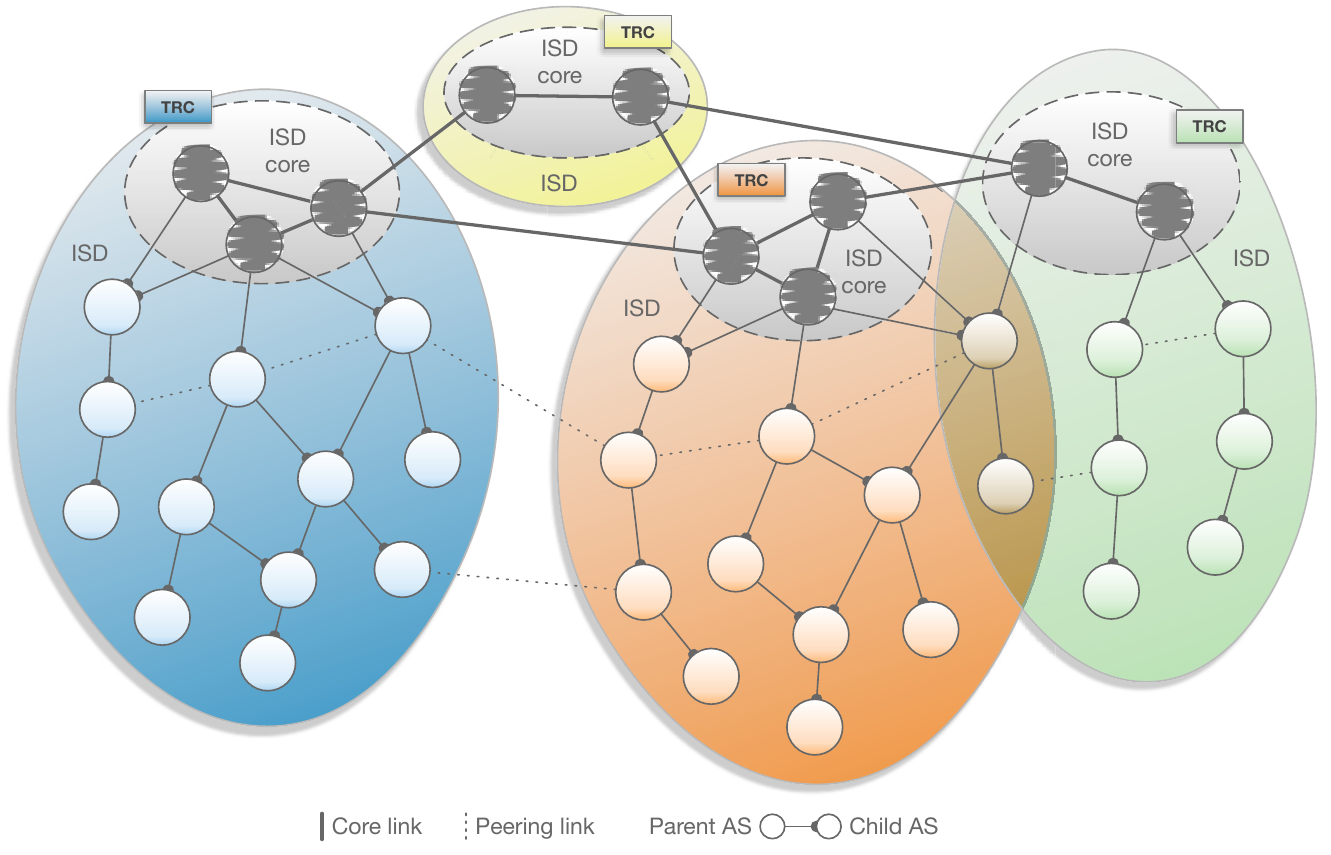
\includegraphics[width=0.75\textwidth]{figures/scion_isd_architecture.png}
    \caption{SCION Architecture with ISD and ASes, where ASes are represented by circles \cite[Chapter 2]{Perrig2022}.}
    \label{fig:scion_isd_architecture}
\end{figure}


\subsection{Core Concepts}
In the following we explain SCION's core features and how it achieves them.
\subsubsection{Isolation}

SCION implements robust isolation through the concept of isolation domains, which are designed to provide both fault and trust isolation.

The configuration of an ISD is stored in a signed file called trust root configuration (TRC).
The TRC includes essential components such as root certificates and policies, which define the trust relationships and operational parameters within the ISD.
In the event of a misconfiguration or failure within an ISD, the impact is contained within that specific domain.
This containment ensures that the rest of the Internet continues to operate unaffected.

In terms of trust isolation, SCION ensures that only the core ASes within an ISD are trusted.
This approach eliminates the potential risks associated with external trust dependencies.
This strategic segregation of trust domains guarantees that issues or breaches occurring within one ISD do not compromise the integrity, or trustworthiness of the whole Internet.


\subsubsection{Control}

SCION allows users to request and select the optimal paths for their network traffic to reach the desired destinations.
A network path can contain up to three path segments, called up-, core- and down-segment.
The up-segment is the path from the source to its core AS, the core-segment is the path between core ASes and the down-segment is the path from the destination core AS to the destination.
These segments are combined to form a path that the packets will traverse.
This allows users to avoid certain regions or countries they do not trust and that may perform some sort of traffic analysis.

Users are not limited to a single path.
With the option to utilize multiple paths simultaneously, SCION empowers users with greater control and flexibility over their network traffic.
This multipath feature also ensures higher availability in case of a network issue along a path.


\subsubsection{Scalability}

The path information in SCION packets is stored in the SCION packet header.
Based on this information, the SCION routers can forward the packets to the next hop without storing any state information or performing expensive longest prefix matching as traditional IP routers do.
The concept of ISD impacts also the scalability of SCION.
It allows splitting up the routing processes into two levels:
One for routing within an ISD and one for routing between ISDs.


\subsection{Services}
This section discusses the main services of SCION.

The \textbf{border router} sits at the edge of an AS and forwards outgoing SCION packet to neighboring remote ASes or incoming packets within the local AS.
To support legacy end hosts that are not able to communicate over SCION, the \textbf{SCION-IP gateway (SIG)} is used.
It translates SCION packets to IP packets and vice versa.
SCION-enabled end host run the \textbf{SCION daemon} and the \textbf{SCION dispatcher}.
The dispatcher is responsible for sending and receiving SCION packets, whereas the main task of the daemon is to fetch path information.

The \textbf{control service} is generic term for the following other services that run in an AS:
The \textbf{beacon service} is responsible for path exploration and the \textbf{path service} for path registration, as well as providing path lookup services to end hosts.
Key management and signature validation is done by the \textbf{certificate service}.


\subsection{Control Plane}
\label{sec:control_plane}

The control plane in SCION is responsible for discovering network path segments.
These segments are verified using AS certificates.
In the following, path exploration and its security mechanisms are explained.
For simplicity, we will only focus on control plane packets within an ISD and not between core ASes of different ISDs.
The interested reader can find more information in Chapter 4 of the SCION book \cite{Perrig2022}.

\subsubsection{Path Exploration}
Path segments are discovered by using path-segment construction beacons (PCBs).
These are special control plane packets that are always originated by a core AS and subsequently propagated to non-core child ASes.
During this traversal, PCBs gather information about the path (e.g., the crossed interfaces at the border routers) and the ASes traversed.
Within an AS, the beacon service verifies the structure and authenticity of the PCB.
If the PCB is validated successfully, it stores the PCB in its local database.
The beacon service then selects the best combination of PCBs and forwards them to the beacon service in a next AS, thereby continuing path exploration.
This process, known as beaconing, is depicted in \cref{fig:scion_path_exploration}.

\begin{figure}[h]
    \centering
    \includegraphics[width=0.75\textwidth]{figures/scion_beacon.png}
    \caption{Propagation of PCBs within an AS \cite[Section 2.3.1]{Perrig2022}.}
    \label{fig:scion_path_exploration}
\end{figure}

\subsubsection{PCB Format}
Formally, a PCB is structured as follows:
$$ PCB = \langle INF \parallel ASE_0 \parallel ASE_1 \parallel \ldots \parallel ASE_n \rangle $$

The PCB comprises an info field $INF$ and a series of AS entries $ASE_i$, where each $ASE_i$ contains all path-related information for the $i$-th traversed AS.
The info field is defined as:
$$ INF = \langle Flags_{INF} \parallel SegID \parallel TS \rangle $$

Here, $Flags_{INF}$ represents various flags used primarily in the data plane during packet forwarding, $SegID$ is a random segment ID, and $TS$ denotes the timestamp indicating when the PCB was created.

For the AS entry, we use a simplified format to highlight the key fields.
A detailed description of the full format can be found in Section 4.1.1.2 of the SCION book \cite{Perrig2022}.
The simplified AS entry format includes of a hop field $HF$ and a signature $\Sigma$.
The format of the hop field is as follows:
\begin{align*}
    HF = \langle &Local \parallel Next \parallel Flags_{HF} \parallel ExpTime \parallel \\  
    &ConsIngress \parallel ConsEgress \parallel HFAuth\rangle 
\end{align*}

$Local$ is the ISD-AS identifier of the AS, $Next$ is the ISD-AS identifier of the next AS in the path (i.e., where the PCB is forwarded next).
$Flags_{HF}$ indicates different processing options for the AS.
The $ExpTime$ field specifies for how long the hop field is valid.
The ingress and egress interfaces (in direction of construction/beaconing) are stored in $ConsIngress$ and $ConsEgress$ respectively.
The hop field is authenticated using the $HFAuth$ field, which is a message authentication code (MAC).
In \cref{sec:mac_calc} we will explain how this MAC is calculated and used.

The signature field $\Sigma$ is used to authenticate the AS entry and is calculated using the private key $K_i$ associated with the AS's public key, which is validated by the certificate of the AS.
The signature is computed over the info field, all previously traversed AS entries, and the current hop field, or formally expressed as:
$$\Sigma_i = \text{Sign}_{K_i} \bigl( INF \parallel ASE_0 \parallel \dots \parallel ASE_{i-1} \parallel HF_i \bigr)$$

\subsubsection{MAC Calculation}
\label{sec:mac_calc}
As previously mentioned, the $HFAuth$ value authenticates the hop field.
This section illustrated how the MAC value also authenticates all previously traversed hops.

Consider a PCB traversing the ASes $AS_0, \dots, AS_n$ with their corresponding secret keys $K_0, \dots, K_n$
The core AS $AS_0$ initiates the beaconing process by sampling a random value, i.e., the segment identifier:

$$ SegID = \beta_0 = Random() $$

Using this value, each AS computes its hop field MAC as follows:
\begin{align*}
    \sigma_i    &= \text{MAC}_{K_i}(\beta_i, TS, ExpTime_i, ConsIngress_i, ConsEgress_i) \\
    \beta_{i+1} &= \beta_i \oplus \sigma_i[0:16] \\
    HFAuth_i &= \sigma_i[0:48]
\end{align*}

Here, $\oplus$ denotes the bitwise XOR operation, and the notation $X[a:b]$ refers to the substring of $X$ from index $a$ (inclusive) to $b$ (exclusive), where the values represent the bit positions.
The hop field authenticator is truncated to 6 bytes to minimize communication overhead.
Additionally, only $\beta_0$ is stored in the $SegID$ field of the PCB, as the other $\beta_i$ values can be recomputed based on $\beta_0$ and the $HFAuth$ values of the previous hop fields.

Recalculation of these values during packet forwarding in the data plane would be too expensive.
Therefore, each router continuously updates the $SegID$ to reflect the value of $\beta_{i+1}$, which the next router uses to calculate its MAC value.

\subsubsection{Path-segment Registration}
Path segments are derived from PCBs and must be registered first before they can be utilized by the end hosts.
From the stored PCBs, the up- and down segments get created:
Since these path segments start or end at the local AS, the selected PCB has to be modified accordingly:
The $Next$ field and the $ConsEgress$ field in the hop field are cleared, and afterwards, the MAC is recomputed on these modified PCBs.
The up-segments are forwarded to the local path service, while the down-segments are sent to the path service of the core AS that originated the PCB.

\subsubsection{SCION Control Message Protocol (SCMP)}


The SCION Control Message Protocol (SCMP) is analogous to ICMP and is used for reporting error and informational messages in SCION networks.
The different types of SCMP messages are shown in \cref{fig:scmp_message_types}.

\begin{figure}[h]
    \centering
    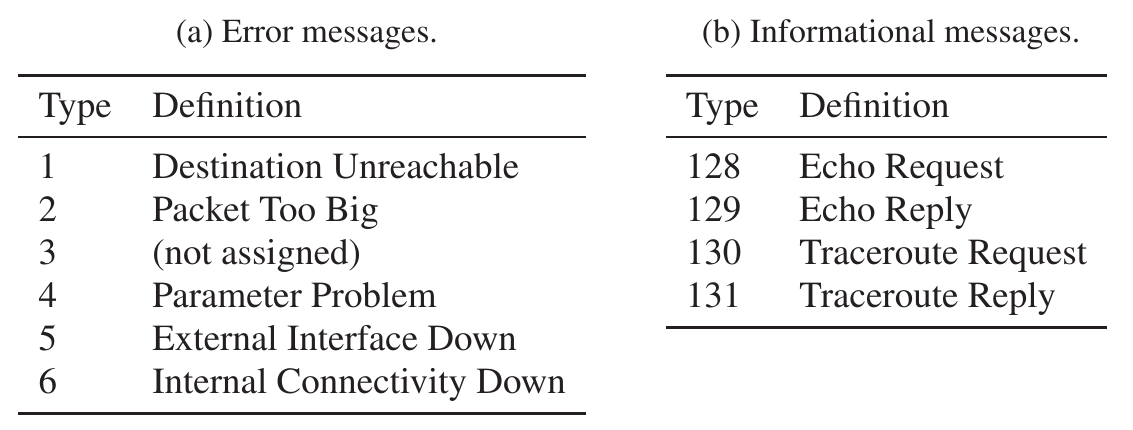
\includegraphics[width=0.75\textwidth]{figures/scmp_message_types.png}
\caption{Different types of SCMP messages \cite[Section 4.7.2]{Perrig2022}.}
    \label{fig:scmp_message_types}
\end{figure}

These messages deliver important information to end host, enabling actions such as network traffic optimization, path switching, and MTU modification.
Given that these messages can lead to significant decisions, their authentication is crucial.
The SCION specification mandates that all SCMP error messages must be authenticated with DRKey (see \cref{sec:drkey} for more details).
Authentication on SCMP informational messages is optional; however, responses must be authenticated if and only if the request was authenticated.

\subsection{Data Plane}
Delivering network packets in SCION between end hosts is managed by the data plane.
It is path-aware and utilizes the path information embedded in the packet header to forward the packets to the next hop.
This section first describes the packet format and subsequently addresses how the path header is constructed and reversed.
Finally, the processing steps at the routers are explained.

\subsubsection{Packet Format}
SCION packets contain a network-layer (layer 3) SCION header, which is structured as depicted in \cref{fig:scion_header_format}.

\begin{figure}[h]
    \centering
    \renewcommand{\arraystretch}{1.5} % Adjust the value to increase/decrease spacing
    \begin{tabularx}{0.5\textwidth}{|>{\centering\arraybackslash}X|}
        \hline
        Common header \\
        \hline
        Address header \\
        \hline
        Path header \\
        \hline
    \end{tabularx}
    \caption{SCION header format \cite[Section 5.2]{Perrig2022}.}
    \label{fig:scion_header_format}
\end{figure}

The SCION common header includes fields needed to process the next headers including details such as header and packet length, the type of the path header, as well as the source and destination address types.

The address header contains the ISD and AS identifiers along with the host addresses of the source and destination.

The SCION path header specifies the path information required for packet forwarding.
We will only focus on the SCION path type, as it is the most common one.
Its structure is shown in \cref{fig:scion_path_header} and starts with a path meta header, 

$$ PathMetaHdr = \langle CurrINF \parallel CurrHF \parallel Seg0Len \parallel Seg1Len \parallel Seg2Len \rangle $$

followed by the info fields and hop fields.
The path meta header consists of the indices of the current info field $CurrINF$ and hop field $CurrHF$, as well as the lengths of the up-, core- and down-segments ($Seg0Len$, $Seg1Len$, $Seg2Len$ respectively).

\begin{figure}[h]
    \centering
    \renewcommand{\arraystretch}{1.5} % Adjust the value to increase/decrease spacing
    \begin{tabularx}{0.5\textwidth}{|>{\centering\arraybackslash}X|}
        \hline
        Path meta header \\
        \hline
        Info field (up) \\
        \hline
        Info field (core) \\
        \hline
        Info field (down) \\
        \hline
        Hop field \\
        \hline
        \cdots \\
        \hline
        Hop field \\
        \hline
    \end{tabularx}
    \caption{Structure of the SCION path header.
    Not all info fields must be present (at least one and at most all three), and their order is fixed \cite[Section 5.4]{Perrig2022}.}
    \label{fig:scion_path_header}
\end{figure}

The flags field in the info field include the $ConsDir$ single-bit flag, which indicates whether the corresponding path segment is traversed in the direction of construction (i.e., beaconing) or in the reverse direction.

\subsubsection{Path Construction and Reversal}

\cref{fig:scion_path_header_contruction} illustrates the construction of the path header from the individual path segments.
Following the path meta header up to three info fields are included.
Their order is fixed and corresponds to the info field of the up-, core-, and down-segments.
Subsequently, the hop fields are added in the order of the path segments.

\begin{figure}[h]
    \centering
    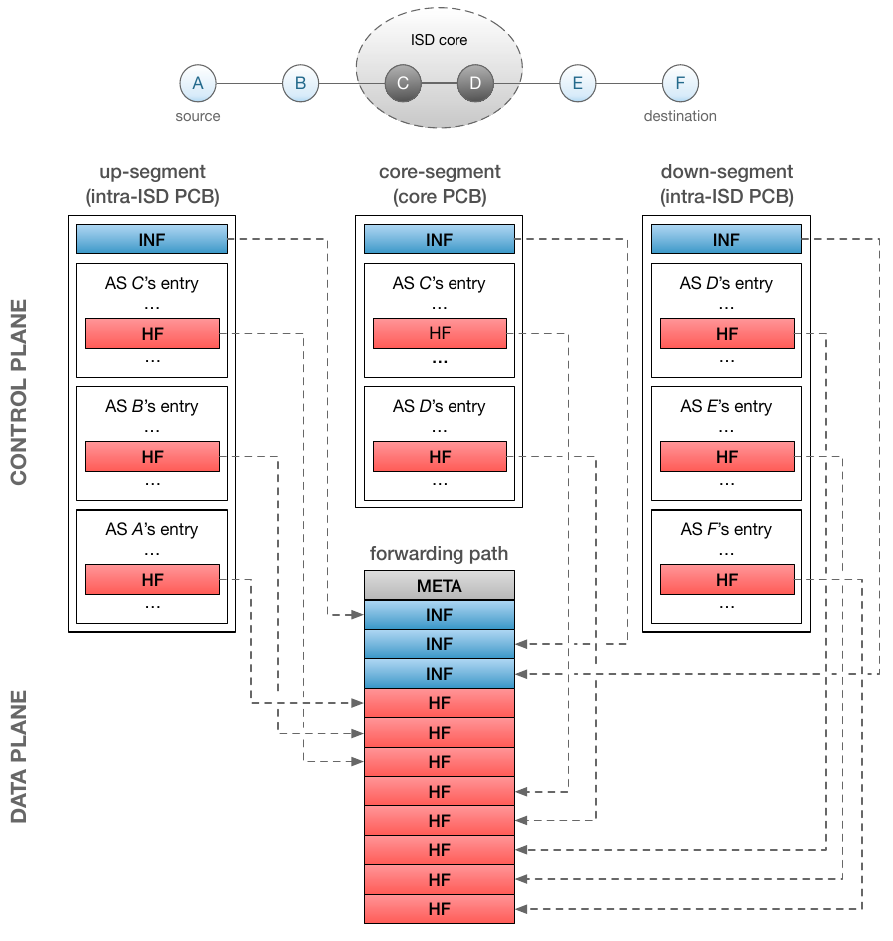
\includegraphics[width=0.75\textwidth]{figures/scion_path_header_construction.png}
    \caption{Construction of the path header out of the path segments \cite[Section 5.4]{Perrig2022}.}
    \label{fig:scion_path_header_contruction}
\end{figure}

When an end host receives a SCION packet, it can use the information in the path header to send a response back to the sender.
In the reply packet, the order of the info and hop fields must be reversed.
Additionally, the $ConsDir$ flag in the info fields has to be flipped, $CurrINF$ and $CurrHF$ should be set to 0, and the order the $SegLen$ fields must be reversed.
This path reversal also allows border routers to communicate any issues encountered during packet processing back to the sender.
Further details on packet processing are explained in the next section.

\subsubsection{Processing at Routers}

The SCION border routers executes various tasks when processing SCION packets and these tasks depend on the position of the router in the path.
The following four router positions are distinguished:

\begin{enumerate}[label=P\arabic*]
    \item In the middle of a path segment
    \item At the joint of two path segments
    \item In the source AS
    \item In the destination AS
\end{enumerate}

Additionally, the specific tasks performed by the router also depend on whether it is an ingress or egress router of the AS.

The tasks for the ingress border router include:
\begin{enumerate}
    \item Ensure that the interface through which the packet was received matches the interface in the current hop field.
    \item Verify that the hop field is not expired and is within its validity period.
    \item Implicitly determine the position of the router in the path based on the header fields (in case of P1, P2, P4).
    \item Perform some general integrity checks on the packet header.
    \item Only in the cases of P1, P2, and P4, and if ConsDir is zero: XOR the $SegID$ of the current info field with $HFAuth$ of the current hop field, i.e., $SegID := SegID \oplus HFAuth$.
    \item Compute $\sigma$ according to the equation shown in \cref{sec:mac_calc}, by using the $SegID$ of the current info field and verify that it matches the $HFAuth$ of the current hop field.
    \item In case of P2: Verify that the segment combination is valid (for example core to down segment is okay, but core to core is not. Check rules in Table 5.1 in the SCION book \cite{Perrig2022} for a complete list of allowed combination).
    Additionally, increment $CurrHF$ and $CurrINF$ by one and verify the second hop field (steps 2 and 6).
    \item In case of P4: Check that the packet header contains the correct destination ISD and AS identifiers.
    \item Finally, encapsulate the packet and forward it to the egress border router (on the interface specified in the current hop field, in case of P1 and P2) or to the destination host (based on the destination address, in case of P4).
\end{enumerate}


The following tasks have to be performed by the egress border router:
\begin{enumerate}
    \item Decapsulate the SCION packet.
    \item Implicitly determine the position of the router in the path based on the header fields (in case of P1 - P3).
    \item Perform some general integrity checks on the packet header.
    \item Check $HFAuth$ of the current hop field (see steps 2 and 6 in the ingress router tasks).
    \item If router is in position P1-P3 and if $ConsDir$ is one: XOR the $SegID$ of the current info field with $HFAuth$ of the current hop field, i.e., $SegID := SegID \oplus HFAuth$.
    \item Increment $CurrHF$ by one.
    \item Forward the SCION packet to the neighboring AS/router.
\end{enumerate}


If any verification step fails, the router has to drop the packet and inform the sender about the issue by sending a ``parameter problem'' SCMP message back.

Note that the hop field is verified twice in the cases of P1 and P2, once each by the ingress and egress border router.
Although this induces some overhead, it offers several advantages:
The ingress router can drop invalid packets early, thereby conserving forwarding resources.
Validation at the egress router ensures that the packet has not been tampered with during its transit within the AS.


\subsection{Security Mechanisms}
In this section, we will cover the most important security mechanisms in SCION.


\subsubsection{Control Plane PKI (CP-PKI)}
\label{sec:cp_pki}
As mention in the \cref{sec:control_plane}, control plane packets, especially PCB are authenticated and contain a signature.
This authentication relies on the control plane public key infrastructure (CP-PKI) of SCION.
Here, we provide only a brief overview of the CP-PKI; detailed information can be found in Section 3.1 of the SCION book \cite{Perrig2022}.

The root of trust in the CP-PKI is the TRC, which include root certificates.
These are used to verify the certificates of certification authorities (CAs).
CAs issue certificates to ASes, which contain the public key of the AS.
This certificate chain is being used to verify the authenticity of an AS.
Each AS (including its border routers, SCION end hosts etc.) knows the TRC of its ISD and can thus verify the certificates of other ASes within the ISD.
This ensures that only valid and authorized ASes can participate in the SCION network, as PCBs are only accepted if they are signed by a valid AS certificate.

While authentication based on signatures and certificates may work well for the control plane with low packet rates, the data plane with high packet rates requires a more efficient authentication mechanism.
This is where the DRKey comes into play, which is explained in the next section.

\subsubsection{Dynamically Recreatable Keys (DRKey)}
\label{sec:drkey}
This section explains the dynamically recreatable key (DRKey) system \cite[Section 3.2]{Perrig2022} and its application within SCION.
Since it relies on symmetric cryptographic keys, it is much faster than the CP-PKI.
This allows for efficient packet authentication in the data plane at high bandwidths and mitigates the risk of Denial-of-Service (DoS) attacks that could occur with slower asymmetric cryptography.
Nevertheless, the DRKey system uses CP-PKI to establish the initial keys.

In DRKey, one entity is on the so-called fast side, as it can derive the key quickly based on locally stored secrets.
The other entity, on the slow side, first needs to fetch the key by issuing a request through the control plane.
Which entity is on the fast or slow side depends on the application.
Generally, the more critical side, i.e., the side more exposed to attacks, is on the fast side.
For example, the border router generating an SCMP error message due to a packet processing error is on the fast side, and the source end host receiving the SCMP error message is on the slow side.

Consider the setup depicted in \cref{fig:drkey_setup} where the server $S_B$ is on the fast side and the host $H_A$ on the slow side.
\begin{figure}[h]
    \centering
    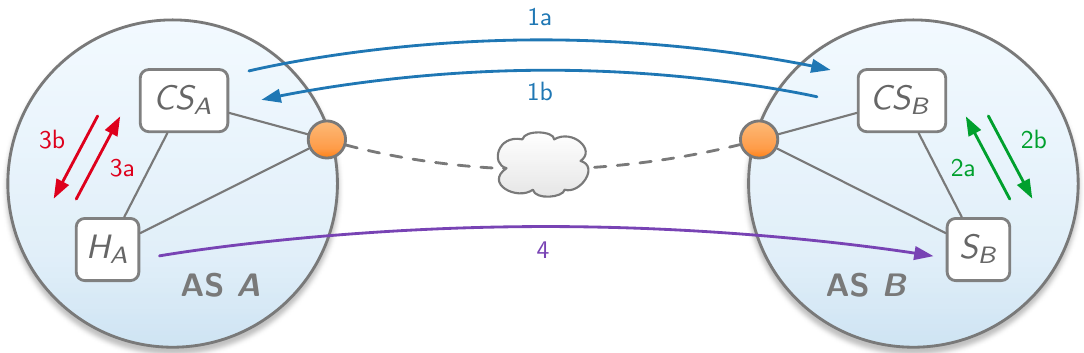
\includegraphics[width=0.75\textwidth]{figures/drkey_topo.png}
    \caption{DRKey communications between an end host and server in different ASes \cite[Section 3.2.2]{Perrig2022}.}
    \label{fig:drkey_setup}
\end{figure}

Each AS selects a randomly generated local secret value, $SV_A$ and $SV_B$ respectively, which is shared to trusted entities within the same AS (e.g., the certificate service).
This secret is used together with a pseudo random function (PRF) by the certificate service in AS B $CS_B$ to derive $K_{B \rightarrow A} = \text{PRF}_{SV_B}(A)$.
The arrow notation indicates that $B$ is on the fast side (it can use the local secret to derive it) and $A$ on the slow side (it has to fetch the key from $B$).
The key fetching of $CS_A$ from $CS_B$ is shown by the arrows 1a and 1b in \cref{fig:drkey_setup}.
Arrows 2a and 2b show that server $S_B$ is trusted and can therefore obtain the secret $SV_B$.
When host $H_A$ wants to authenticate itself to server $S_B$ (arrow 4), it contacts the certificate service $CS_A$ and requests a host-to-host key $K_{B:S_B \rightarrow A:H_A}$, which $CS_A$ can locally derive using $K_{B \rightarrow A}$ (arrows 3a and 3b).
Because $S_B$ is on the fast side, it can derive the key $K_{B:S_B \rightarrow A:H_A}$ using $SV_B$.

\paragraph{Key Derivation}
In the following, we will explain the key derivation process in more detail.
Based on the AS-to-AS key $K_{B \rightarrow A}$, second level keys (host-to-AS or AS-to-host) are derived like this:
\begin{align*}
K_{B \rightarrow A:H_A} &= \text{PRF}_{K_{B \rightarrow A}}(0 \parallel H_A) \\
K_{B:S_B \rightarrow A} &= \text{PRF}_{K_{B \rightarrow A}}(1 \parallel S_B)
\end{align*}

$H_A$ and $S_B$ are the host and server addresses, respectively.
Finally, the third level (host-to-host) key can be derived using the host-to-AS key and by applying the PRF to the slow host's address:
\begin{align*}
    K_{B:S_B \rightarrow A:H_A} = \text{PRF}_{K_{B:S_B \rightarrow A}}(H_A)
\end{align*}

The secrete value $SV$ can be different for different protocols and applications.

\paragraph{SCION Packet Authenticator Option}
\label{sec:spao}
One prominent application that uses DRKey is the SCION packet authenticator option (SPAO) \cite[Section 3.3]{Perrig2022}.
SPAO is added to the SCION header of a data plane packet and provides source authentication between end hosts.
Since even the first packet sent is authenticated, there is no need for explicit key exchange between end hosts.
Additionally, SPAO also provides integrity protection of the packet.
To achieve this, different algorithms are supported.
The specific algorithms and further details on SPAO can be found in the SCION book or on the official documentation website \cite{anapayaSCIONPacket}.


\section{Anapaya}
\label{sec:anapaya}
In this section, we will introduce Anapaya, a company that provides SCION services.
We will also explore the different solutions they offer and how these are used by their customers.

\subsection{Overview}
In 2017, the demand for commercial usage of SCION increased as several Internet Service Providers (ISPs) and entities in the financial sector wanted to adopt it.
As a result, the company Anapaya Systems was founded by the ETH professors Adrian Perrig, David Basin, and Peter Müller.
Since then, the demand for SCION in the industry has continued to grow.
Interest in SCION extends beyond industry to the academic community as well.
The core SCION components are open source, allowing them to be inspected, tested, and used by anyone.
Other components, such as a management system, are exclusively distributed to Anapaya customers \cite{ethzSecureInternet}.


\subsection{Solutions}
In the following, a brief overview of the different Anapaya solutions is provided.
The information is based on the official Anapaya website \cite{anapayaHomepage} and their documentation \cite{anapayaDocs}.
Each of these solutions contain two software packages:
One packages defines the SCION software, its components, and configuration.
The other package includes system configuration, such as installed software and its  specific settings.

\subsubsection{Anapaya CORE}
The Anapaya CORE product is deployed by ISPs that operate a SCION core AS.
Typically, at least two Anapaya CORE devices are deployed to connect to other core ASes and its customers.
Two devices are used to ensure redundancy and high availability and allow performing maintenance on one device without affecting the network.
Anapaya CORE includes the necessary software components to run a SCION core router.
The software is compatible with common x86 of-the-shelf server hardware, but Anapaya also sells pre-configured hardware.


\subsubsection{Anapaya EDGE}
Anapaya EDGE is typically deployed by end customers, such as enterprises or data centers.
It provides an entry point to the SCION network and are primarily used to connect to the SCION core routers.
The Anapaya EDGE product implements the SCION border router functionality together with the SCION-IP gateway.
This allows both SCION-enabled and legacy end hosts to use the SCION network and benefit from its benefits.
The solution also includes a management system that enables customers to define their communication partners.
It allows prioritizing certain paths through configured traffic policies.

\subsubsection{Anapaya GATE}
The Anapaya GATE solution is operated by ISPs and incorporates the SCION-IP gateway module.
It allows companies to announce certain services exclusively on the SCION network, thereby preventing DDoS, intrusion, and other attacks from the traditional Internet.
Typical users of the Anapaya GATE product include employees working from remote or trusted parties who otherwise do not have SCION access.
These trusted users are directed to the Anapaya GATE of the ISP, which then forwards the traffic to the Anapaya Edge of the end customer.
Communication from remote users to the Anapaya GATE use standard IP traffic, whereas communication between the Anapaya GATE and the Anapaya Edge is done over SCION.

\subsection{Cyber-Defence Campus}
The Cyber-Defence (CYD) Campus is also a customer of Anapaya and uses SCION for their research.
At their locations in Lausanne, Thun, and Zurich Anapaya Edge devices are deployed.
Further details on their SCION network setup can be found in \cref{sec:setup}



\section{Security Testing}
\label{sec:security_testing}
Regular security tests are essential to ensure the security of a system.
This is especially important for systems that are exposed to the Internet, as they face a high risk of being attacked.
By proactively testing the security of a system, vulnerabilities can be identified and fixed before they are exploited by attackers.
In the following, we will provide a general overview of different security testing methods and tools.

\subsection{Automatic Scanning Tools}
Automatic scanning tools offer an easy and efficient method to identify vulnerabilities and misconfiguration of specific software, entire networks or even individual devices.

When scanning devices, many tools are capable of performing both unauthenticated and authenticated scans.
Authenticated scans, which use credentials to log in to the target device, can gather more detailed information about the device and provide more accurate results.
At the end of a scan, these tools generate reports that offer a comprehensive overview of the identified vulnerabilities and weaknesses.
Some tools even provide suggestions for remediation.
Examples of automatic scanning tools include Nessus \cite{nessus} and OpenVAS \cite{openvas}.
The primary difference between these tools is that Nessus is a proprietary, while OpenVAS is open-source.
Both tools are free to use; however, the paid version of Nessus additionally offers the option to run compliance scans.
Compliance scan checks if the target device adheres to specific standards, such as the Center for Internet Security (CIS) benchmarks.

Other tools, such as SSH audit \cite{sshaudit}, focus on specific services, in this case SSH.
They check the configuration of the service and provide recommendations for improving its security.


\subsection{Manual Testing}
Manual testing is a more time-consuming and complex process compared to automatic scanning tools.
While automatic tools provide a good overview of known vulnerabilities and misconfiguration, manual testing can identify more complex issues that are not easily detectable or even not possible to detect by automatic tools.
These include logical errors, custom software, complex setups, dependencies between different systems, and other issues that require human intelligence to find.
This human expertise can uncover subtle weaknesses and nuances in different environments that automated tests might miss.


\chapter{Problem Statement}
\label{ch:problem}

This chapter presents the problem statement of this thesis.
It discusses the security challenges that SCION faces, including the threat model and the impact of attacks.
Finally, it presents the objectives of this thesis.

\section{Fundamental Problem}
\label{sec:fundamental-problem}
In released software products, it is estimated that they contain between 1 and 25 errors per 1,000 lines of code \cite{McConnell2004}.
Despite the SCION protocol being publicly known, investigated by the research community, and partially formally verified \cite[Chapters 7, 22, and 23]{Perrig2022}, there remains a risk of vulnerabilities in the protocol and especially its implementation.
This risk is heightened in the SCION product sold by Anapaya, because it is closed-source and modified to meet industry requirements.
Unlike the open-source version, which relies solely on software for its data plane processing, Anapaya's SCION product uses several acceleration technologies \cite{anapayaPerformanceOptimizations}.
These modifications could introduce new vulnerabilities that are not present in the open-source version, eluding the thorough analyses conducted previously.

Even if the implementation of SCION were flawless and contained no bugs, its security would be rendered meaningless if the devices running the software were not properly secured.
Insecure devices could be compromised, undermining the integrity of SCION itself.
Potential attacks include disruption of SCION communication, packet manipulation, and data exfiltration.
Moreover, attackers could silently update the SCION software to a malicious version containing backdoors or other vulnerabilities, enabling undetected compromises of the entire network.
Given that Anapaya sells devices running their version of SCION, ensuring the security of these devices is crucial.
This is especially important since these devices are deployed in production environments, making them attractive targets for attackers.
Proper security measures must be in place to protect these high-value targets from potential threats.

Even with a flawless SCION implementation and robustly secured devices, the network remains susceptible to fundamental and pervasive threats such as volumetric attacks.
Volumetric attacks overwhelm network resources by flooding the target with a high volume of traffic, rendering legitimate communication impossible.
These attacks exploit the underlying infrastructure rather than specific software vulnerabilities, highlighting that even the most secure protocol and devices are not immune to such brute-force tactics.

\section{Attacker Models}
\label{sec:attacker-models}
This section covers potential attacker models, their capabilities, and the specific threats they pose to the SCION network and its implementation.

\subsection{Malicious SCION End Host}
A malicious SCION end host refers to an adversary with legitimate access to the SCION network who operates an endpoint within an AS.
This attacker can generate, send, and receive SCION packets, potentially exploiting weaknesses in the protocol or its implementation.
Such an attacker could attempt to manipulate packet headers, inject malicious payloads, or exploit known vulnerabilities in the SCION software.
Additionally, they could exploit misconfigurations or weak security controls on SCION services running in the AS.
By doing so, they might disrupt communication, corrupt data integrity, or exfiltrate sensitive information.
The threat posed by a malicious end host is significant due to their legitimate access and ability to masquerade malicious activities with regular network traffic.

\subsection{On-path Attacker}
An on-path attacker, also known as a man-in-the-middle (MitM), is positioned on the communication path between two SCION entities.
They are capable of intercepting, monitoring, blocking, replaying, and modifying packets in transit.
On-path attackers can exploit weaknesses in the SCION protocol to redirect traffic, conduct traffic analysis, or inject malicious data into the communication stream.
They can also carry out sophisticated attacks such as session hijacking and traffic manipulation.
The impact of an on-path attacker can be severe, leading to compromised confidentiality, integrity, and availability of communications.

\subsection{Off-path Attacker}
An off-path attacker does not have direct access to the communication path between SCION nodes but can still attempt to disrupt or compromise communications through indirect means.
This attacker might use techniques such as spoofing, reflection attacks, or exploiting vulnerabilities in routing protocols to influence the SCION network.
Although they lack the direct interception capabilities of an on-path attacker, off-path attackers can still cause significant disruptions by misleading network elements, redirecting traffic, or causing congestion.
The effects of an off-path attacker include potential network outages, reduced performance, and indirect data compromise.
\newpage
\subsection{Non-SCION Adversary}
A non-SCION adversary represents a threat actor who has no access to SCION and thus can not directly interact with the SCION network.
Such an attacker might target the physical infrastructure supporting the SCION network, including routers, servers, and other hardware components.
They could exploit vulnerabilities in the underlying operating systems, firmware, or hardware to disrupt SCION operations or compromise the network.
Additionally, they could attempt to disrupt the network through distributed denial-of-service (DDoS) attacks, aiming to exhaust resources and render the network unavailable to legitimate users.
The threat from external attackers is significant as they can cause widespread disruptions, impacting the availability and performance of the SCION network.



\section{Thesis' Objectives}
As mentioned in \cref{sec:fundamental-problem} the security of Anapaya's version of SCION mostly depends on the security of their modified SCION data plane implementation and of the devices they sell.
This thesis aims to improve the security of Anapaya's SCION product by addressing the following objectives:

\begin{itemize}
        \item \textbf{Security of Operational Devices:}
        We conduct an in-depth security assessment of the devices running Anapaya's version of SCION.
        This includes identify potential vulnerabilities and provide recommendations for mitigating these risks.
        A particular emphasis is placed on attack vectors that can be exploited by remote attackers who do not have direct access to the devices (i.e., do not have physical access nor login credentials).

        \item \textbf{SCION network in use:}
        We evaluate the SCION implementation in Anapaya's products to uncover any weaknesses or vulnerabilities that could be exploited by attackers.
        Using the attacker models presented in \cref{sec:attacker-models}, we assess the impact of potential attacks on the SCION network.
        The goal is to provide insights into the security of the SCION protocol and its implementation in real-world scenarios.

        \item \textbf{Impact of Volumetric Attacks on SCION:}
        Our last objective aims to investigate the impact of volumetric attacks on the SCION network, specifically assessing how such attacks affect SCION's performance and availability.
        The analysis will include attacks originating both from the traditional Internet and within the SCION network itself, examining their potential to disrupt SCION's operations.
        Furthermore, the objective includes identifying and evaluating mitigation strategies to enhance SCION's resilience against these volumetric threats, ensuring robust protection of the network's critical infrastructure.
\end{itemize}




\chapter{Methodology}
\label{ch:methodology}

This chapter outlines the methods used to analyze the security and potential vulnerabilities of the Anapaya version of SCION.
The general approach is presented in \cref{sec:general-approach}, followed by the concrete setup used in the assessment in \cref{sec:setup}.
\cref{sec:analysis-methods-tools} provides an in-depth look at the methods and tools used in the analysis.
Finally, \cref{sec:methodology:disclosure} describes the disclosure process with Anapaya.


\section{General Approach}
\label{sec:general-approach}
The general approach of this thesis focuses on a comprehensive analysis of the security features and potential vulnerabilities of the Anapaya version of SCION.
Given its proprietary nature, this research employs a combination of exploratory and analytical approaches.

\subsection{Exploratory Approach}
The exploratory approach is utilized in this research to address the limited public knowledge about Anapaya's version of SCION.
As this version incorporates proprietary modifications that are not fully publicly documented, an exploratory approach is essential for uncovering and understanding these new or undocumented features.
The exploratory phase involves conducting preliminary investigations to identify potential vulnerabilities, security features, and other relevant aspects of the implementation.
This includes a review of available documentation, security scans, and configuration checks to gather initial data on the system.

These early finding from exploratory efforts will guide the subsequent analytical phase of the research, providing a foundation for more in-depth analysis and testing.

\subsection{Analytical Approach}
The analytical approach is employed to systematically evaluate and interpret the security characteristics identified during the exploratory phase.
This approach is crucial for conducting a detailed analysis of the security mechanisms and potential vulnerabilities within the Anapaya SCION environment.
It involves a detailed examination of the identified security mechanisms, potential vulnerabilities, and their implications for the overall security of the SCION network.
The goal is to move beyond initial discovery to a deeper understanding and rigorous assessment of security aspects.


\section{Setup}
\label{sec:setup}
The security analysis is conducted against the SCION deployment at the CYD Campus locations.
A simplified network setup is shown in \cref{fig:network-setup}.
Each CYD Campus location forms its own AS and includes an Anapaya EDGE device.
The three ASes are connected via three different Core ASes to the SCION production network.
In each of these CYD Campus ASes, we deploy a Kali virtual machine (VM) that runs the SCION end host code, enabling interaction with the SCION network.
At ETH Zürich, SCION access extends beyond the CYD Campus, where we operate an additional Kali VM.
To assess the influences of the traditional Internet on SCION, we also have access to a non-SCION VM in the ETH Zürich network.
According to the service offer from SWITCH the traditional Internet and SCION connection in Zürich are physically separated.
At the other CYD Campus locations, no such separation information is provided.

\begin{figure}[h]
    \centering
    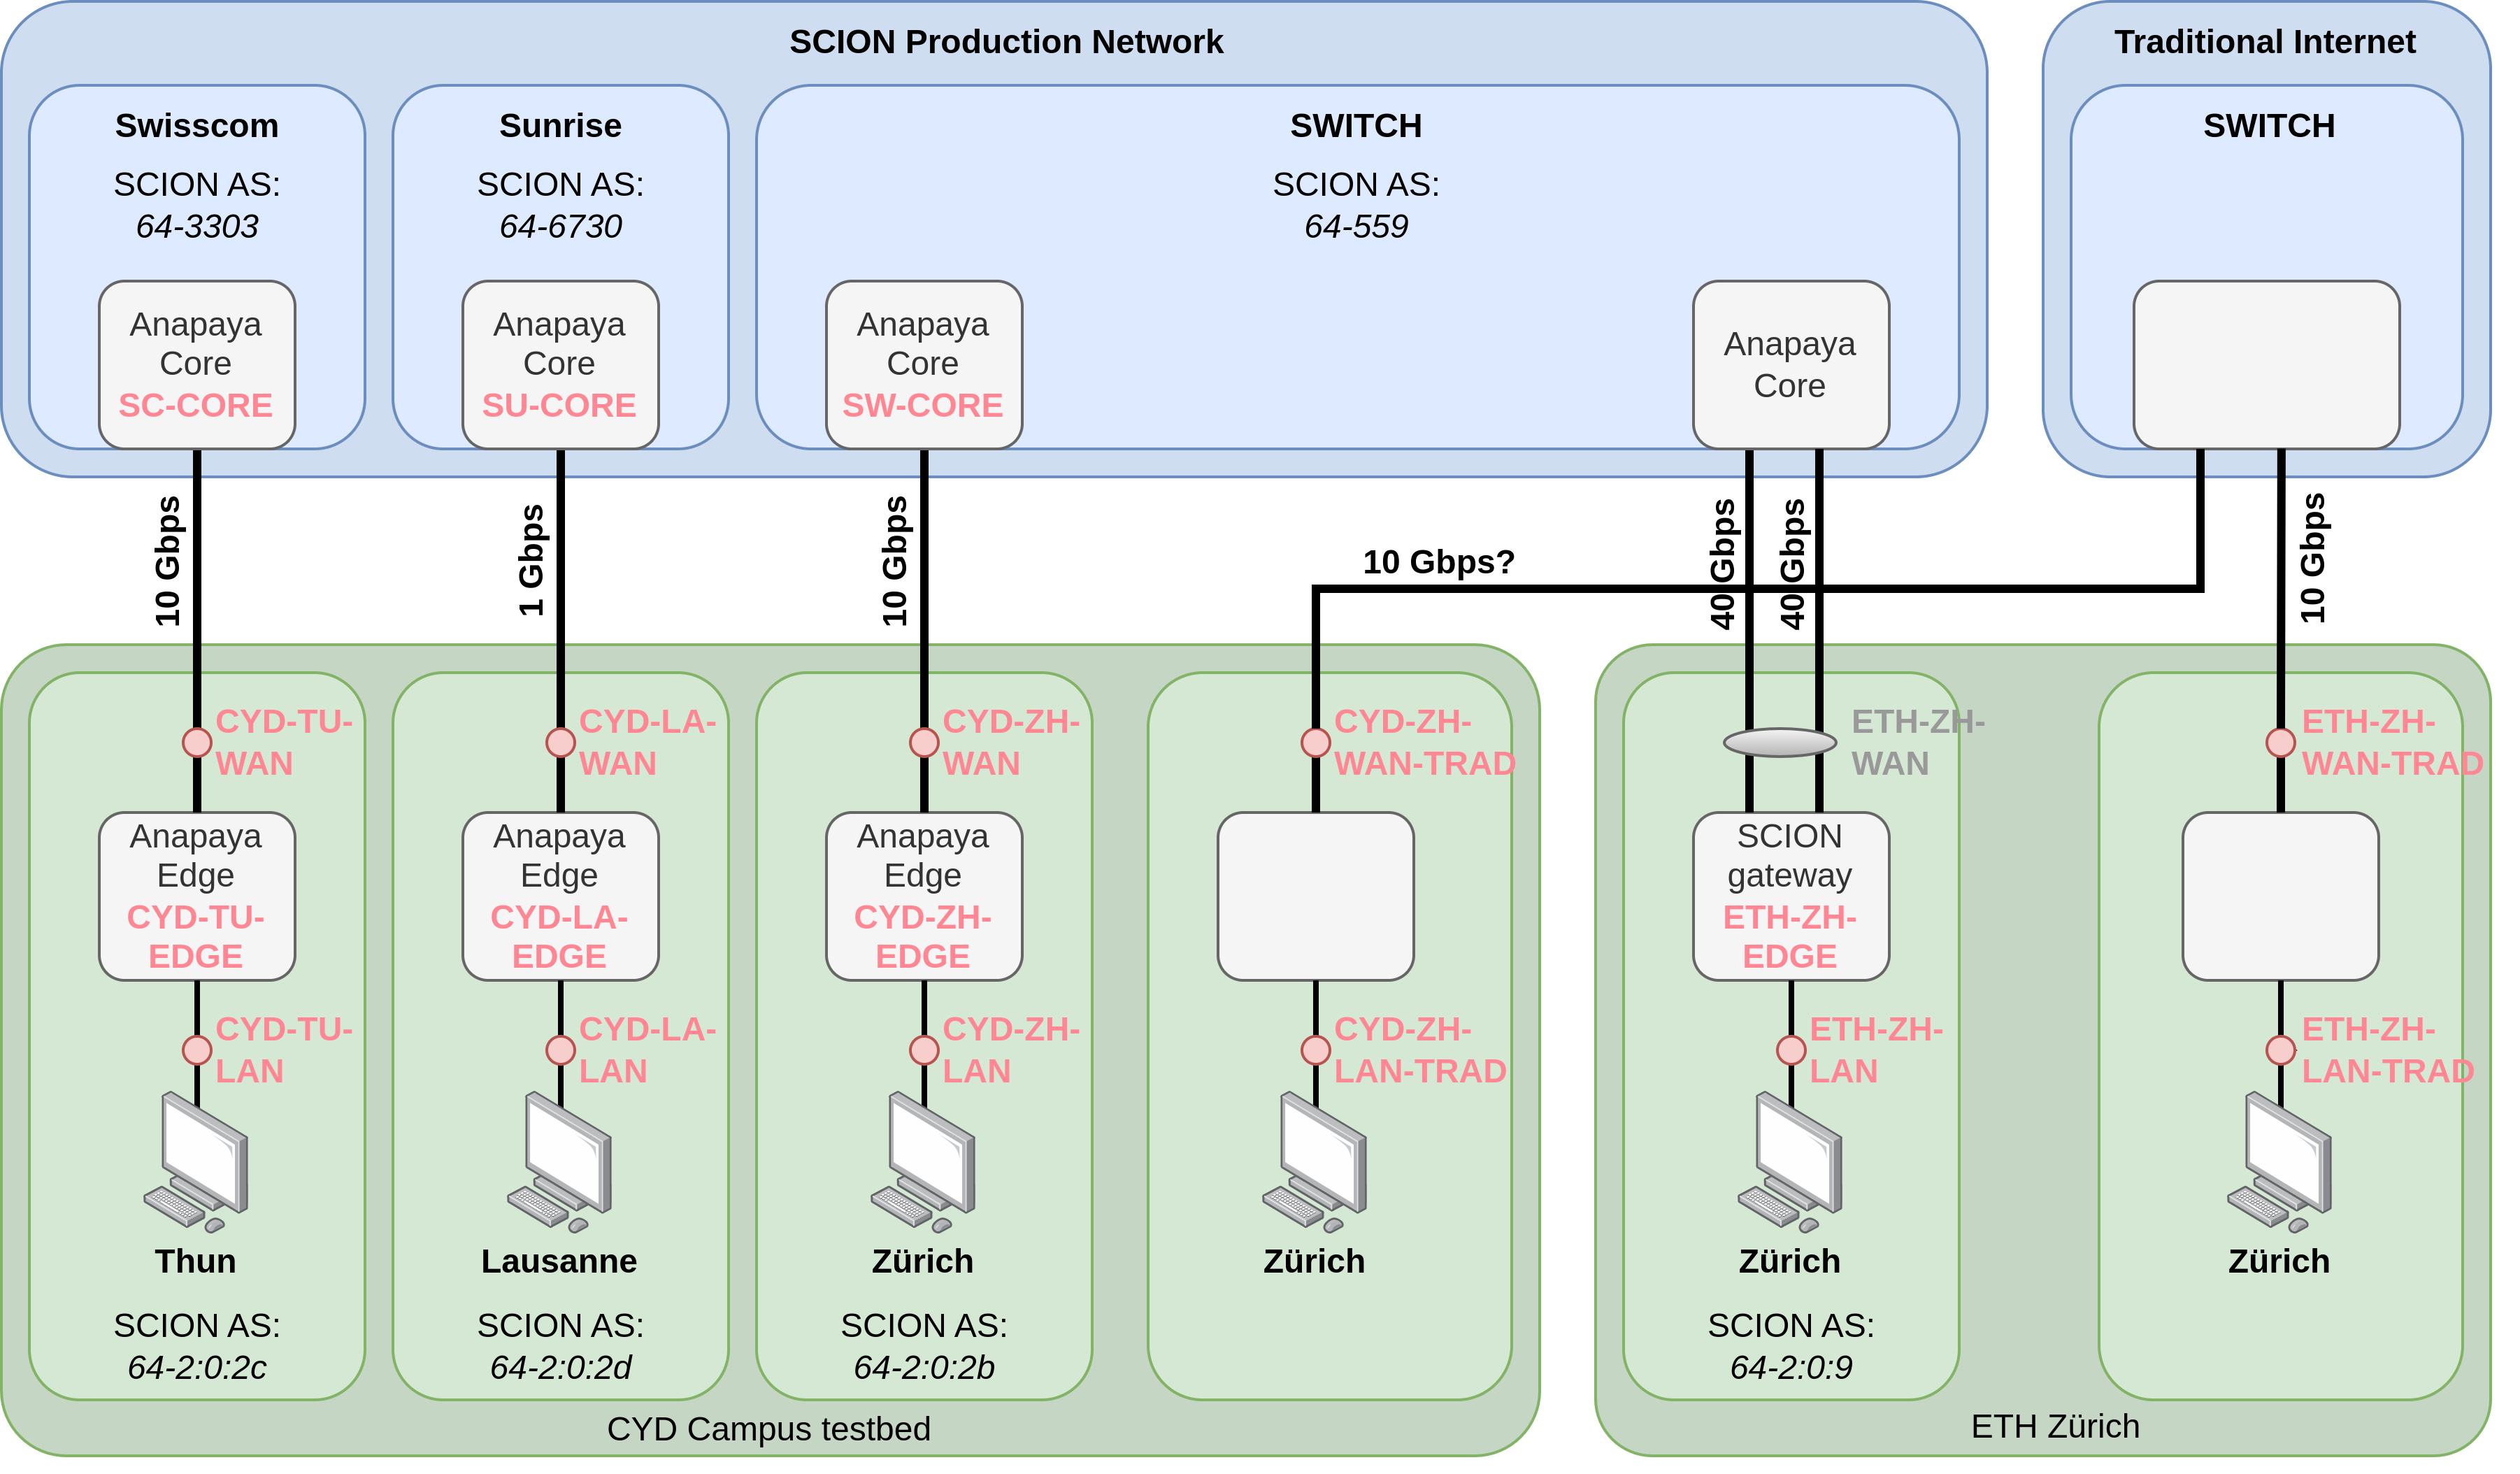
\includegraphics[width=\textwidth]{figures/scion_setup2.drawio.png}
    \caption{Network Setup during the Security Assessment}
    \label{fig:network-setup}
\end{figure}

Additionally, apart from these operational devices, CYD Campus acquired another Anapaya device.
It is not part of the SCION production network and only used for offline testing purposes.

\newpage
\section{Analysis Methods and Tools}
\label{sec:analysis-methods-tools}
This section outlines the methods and tools used to conduct the security analysis of the Anapaya EDGE devices.

\subsection{Automatic Scans}
To conduct our exploratory analysis, we employ automated scanning tools to identify potential vulnerabilities and security weaknesses in the deployed Anapaya devices.
The popular tools \textbf{Nessus} and \textbf{OpenVAS} give an initial overview of the security posture of the devices by scanning for known vulnerabilities and misconfigurations.
Nessus is also being used to perform a compliance audit to check if the devices adhere to security best practices and standards, such as CIS benchmarks.
An \textbf{SSH audit} is conducted to identify potential weaknesses in the SSH configuration of the devices.
Furthermore, running software and services are analyzed using tools like \textbf{systemd-analyze} \cite{systemdAnalyze} and \textbf{Docker Trivy} \cite{trivy}.


\subsection{Manual Investigations}
Complementing the automated scans, manual investigations include reviewing the findings of the automated tools and conducting in-depth analysis of specific areas.
In addition, we review manually the software and configurations detected by the automated scans.

Apart from the device itself, everything related to the SCION protocol is manually checked.
This includes the SCION management system, and all SCION network interactions.
How we capture and analyze these interactions is described in the next section.


\subsection{Data Collection and Modification}
During the security analysis, network packets are generated, captured, analyzed, and modified.
This is done to observe and reason about network flows, for example to check if a reflection attack worked or not.
Furthermore, if our generated packets cause SCMP error messages, we can reason about the correct behavior or can also use this information to analyze and revise our generated packets.
We use \textbf{Wireshark/tshark} \cite{wireshark} for packet capture because there already exists a SCION plugin for Wireshark, which allows us to dissect SCION packets \cite{wiresharkSCION}.
To generate and modify SCION packets, the tools \textbf{scapy} \cite{scapy} with its SCION extension \cite{scapySCION} are used.
It allows to easily define correctly formatted SCION packets and modify them as needed.

\newpage

\subsection{Volumetric Data Generation}
We assess the robustness of SCION by conducting volumetric denial-of-service attacks.
The primary objective of such an attack is to saturate the target's network bandwidth, overwhelming it with a large volume of data packets.
For generating the volumetric data, we use the TRex traffic generator \cite{trexWebsite}, a versatile and high-performance tool capable of simulating both stateful and stateless traffic.
TRex allows customizing traffic parameters, enabling us to closely mimic real-world attack scenarios.
We configure TRex to send a continuous stream of large data packets, thereby maximizing the use of on network resources.
This approach allows us to evaluate the resilience of the SCION architecture under severe traffic conditions, offering valuable insights into its performance and robustness.

\section{Disclosure Process}
\label{sec:methodology:disclosure}

The disclosure process followed a structured and collaborative approach with Anapaya to ensure both thorough evaluation and responsible communication of findings.
Initially, we conducted independent penetration tests on the SCION infrastructure at the CYD Campus to identify potential security vulnerabilities and assess their impact.
This independent assessment aimed to provide an unbiased analysis of the system.
Following these tests, we held a discussion with Anapaya to share our preliminary findings and to obtain their insights and feedback.
Anapaya then implemented necessary software updates to address the identified weaknesses and vulnerabilities.
They were also given the opportunity to review and comment on the findings.
We incorporated their feedback into the final report, ensuring that their perspectives and any additional insights were accurately reflected.
Finally, Anapaya approved the publication of the results, allowing us to share the outcomes of the security analysis with the broader community.


\chapter{Implementation}
\label{ch:implementation}

% Describe the architecture of your implementation and explain the choices you made.
% Why did you use library X instead of Y?

In this chapter, we present our implementation of the different components that we used to conduct our experiments.
We will first describe the setup and configuration of the Kali machines, as well as the use of the open-source SCION implementation.
Subsequently, in \cref{sec:impl:SCIONpackets}, we will explain the processes for generating and modifying SCION packets.
\cref{sec:impl:attackerModel} details the implementation of the different attack models.
Finally, \cref{sec:impl:VolumetricDoS} explains how we conducted the volumetric denial-of-service attacks.

\section{Kali Machines}

The Kali virtual machines mentioned in \cref{sec:setup} contain numerous tools and software for performing penetration tests.
We upgraded these machines to include all the additionally needed programs that were listed in \cref{sec:analysis-methods-tools}.

To interact with SCION, we installed the SCION end host stack on the Kali machines.
This stack includes a general \texttt{scion} helper binary, the SCION dispatcher, and the SCION daemon, all of which we built from the open-source code.
The \texttt{scion} binary is a tool that facilitates interaction with the SCION network.
It can be used to send SCMP echo requests (i.e, SCION pings) or perform traceroutes to a specific destination.
The binaries require configuration files to connect to the SCION network.
For example, the addresses and interfaces of the AS-local border routers must be known, or the TRC of the whole ISD is required.
We extracted the necessary configuration files from the Anapaya EDGE devices, copied them to the Kali machines, and attempted to run the SCION end host stack.
This attempt was unsuccessful because Anapaya uses a different format for the configuration files than the open-source SCION implementation.
After some manual adjustments, we managed to get the dispatcher and daemon running and connected to the SCION production network.

At this point, we were capable of sending and receiving SCION packets to and from any other SCION device in the network.
Additionally, this setup allowed us to fetch all possible path information to a specific destination using the \texttt{scion} binary with the \texttt{scion showpaths} command.


\section{Open-Source SCION}
We utilize the open-source code not only to build the end host stack, but also to verify the behavior of the Anapaya's proprietary SCION implementation.
By leveraging the open-source code, we can validate certain hypotheses and determine if specific features are implemented identically or were modified by Anapaya.


\section{SCION Packets}
\label{sec:impl:SCIONpackets}
Typically, SCION packets are not directly accessible to the user as they are generated and sent by a SCION application, such as the \texttt{scion} binary.
However, for our experiments, we needed to generate and modify custom packets.
The Python library scapy, with its SCION extension \cite{scapySCION}, facilitates this process.
It allows stacking different headers on top of each other and defining every field of them.
This capability enabled us to generate SCION packets with custom payloads and headers.
To send and receive SCION packets, scapy does not require a running SCION dispatcher or daemon.
Nonetheless, in our implementation, we use the SCION end host stack to fetch the path information, which we then use to generate custom SCION packets with valid path headers.




\section{Attacker Models}
\label{sec:impl:attackerModel}

This section outlines the implementation of the different attacker models.
Their individual capabilities are described in \cref{sec:attacker-models}.

\subsection{Malicious SCION End Host}
We used the Kali machines to simulate a malicious SCION end host.
These machines are integrated into the SCION network and are capable of sending and receiving SCION packets.
This enables us to generate and dispatch custom, potential maliciously crafted, SCION packets to other SCION devices, using the approach mentioned previously in \cref{sec:impl:SCIONpackets}.
Since the Kali machines can also receive and analyze SCION packets, we can verify whether the packets are correctly received and processed by the target devices.
This process allows us to assess whether the target devices are vulnerable to the specific attack.
Additionally, we also have access to our target devices, including all three operational Anapaya EDGE devices, to evaluate the impact of potential attacks.

Moreover, the Kali machines are used to fetch and store path information for future use.
This is necessary because path information is frequently updated and removed, despite the paths remaining valid and not yet expired.
By preserving these path information, we can later send SCION packets with valid path headers (i.e., with correct MAC values) but with potentially expired hop fields.

\newpage
\subsection{On-path Attacker}
A logical approach to implementing an on-path attacker would involve utilizing the three operational SCION devices at the CYD Campus locations.
These devices are present on each path between our SCION end hosts (i.e., Kali machines) and any other reachable SCION device within the network.
This would enable us to intercept, monitor, block, replay, and modify packets in transit.
However, employing these devices would affect other SCION users and their connections.
Due to ethical and legal concerns, we opted against using these devices for our experiments.
Moreover, even in the absence of these concerns, implementing an on-path attacker on these devices would be challenging, particularly due to the need for custom software installation.

Instead, again the Kali machines are used to simulate an on-path attacker.
We configure a socket through which an end host can send and receive SCION packets.
On the same machine, a custom Python script operates on the other side of the socket to simulate the on-path attacker.
In the absence of an attack, this script simply forwards received SCION packets to the border router and sends the corresponding response back to the end host via the socket.
During an attack, the script has the capability to modify, save, or drop both incoming and outgoing SCION packets.



\subsection{Off-path Attacker}

The CYD Campus SCION setup, comprising three distinct locations and three separate ASes, facilitates the simulation of an off-path attacker.
In this setup, one location is designated as the attacker, while the other two serve as potential victims.
The attacker is capable of sending SCION packets to the victims but lacks direct access to the communication path between the two.
This way, we can realistically implement an off-path attacker within the SCION production network.
Typically, a Kali machine is employed to simulate an end-host off-path attacker.
In certain scenarios, we also consider the Anapaya device within the attacker's AS as malicious, thereby simulating a fully malicious AS that operates off-path.

\subsection{Non-SCION Adversary}
To simulate an attacker without SCION access, we could utilize any device that is not connected to the SCION network.
For this purpose, we select a device connected to the traditional Internet and located outside the CYD Campus.
ETH Zurich provided access to their network as well as a dedicated server from which we can launch attacks.
An advantage of this setup is that both ETH Zurich and the CYD Campus in Zurich share the same Internet service provider, SWITCH.
This allows for simpler coordination of specific attacks, such as volumetric denial-of-service attacks.

\newpage
\section{Volumetric Attacks}
\label{sec:impl:VolumetricDoS}
This section details the implementation of volumetric denial-of-service attacks to evaluate the resilience of SCION under high traffic loads.
We employ TRex, a state-of-the-art traffic generator, to produce the high volume of traffic required for these attacks.
The setup, located at ETH Zurich, consists of a server equipped with an MT27800 Mellanox 100 Gbit/s network interface card, running TRex version 2.87.
We conducted two types of volumetric attacks:
One from a traditional (non-SCION) Internet adversary and another from a malicious SCION end host.

\begin{itemize}
    \item \textbf{Traditional Internet:}
    To simulate a volumetric attack originating from the non-SCION adversary, we configured TRex to continuously send large UDP packets towards the public IP of the CYD Campus location in Zurich.
    \item \textbf{SCION:} Since TRex does not natively support generating SCION packets, we developed a custom script that creates a valid SCION packet, including the required path information to the border router at CYD Campus Zurich.
    This script stores the packet in a PCAP file, which can then be replayed by TRex.
    Similar to the first attack, the SCION packet contains a large payload to maximize network resource consumption.
    The script is available in our GitHub repository \cite{gitHubMseewerMasterThesis} for reference and use.
\end{itemize}

We were permitted to generate up to 20 Gbit/s of traffic from the ETH network, which exceeds the 10 Gbit/s capacity of the CYD Campus link in Zurich, ensuring that the attack traffic fully utilizes the available bandwidth.

To evaluate the impact of the attack on SCION's performance at the CYD Campus in Zurich, we employed two SCION-specific tools from the measurement point in Thun.
First, we utilize \texttt{scion ping} to assess the reachability of the targeted SCION AS during the attack.
Second, to measure the remaining available bandwidth, we use the \texttt{scion-bwtester} tool.
This provides insights into the degree of resource exhaustion caused by the attack.

We chose Thun as the measurement point due to its superior network infrastructure compared to Lausanne, offering a significantly higher bandwidth capacity (10 Gbit/s vs. 1 Gbit/s).
This selection ensures that any observed performance degradation could be more directly attributed to the DoS attack rather than limitations in the network infrastructure.
\chapter{Findings}
\label{ch:findings}

% * Repeatable, specific description
% * Provide intuition, key idea
% * State what the problem is that you want to address in that section
% * Describe all parts of life cycle: setup, run, maintenance, etc.
% * Explain with an example (together with the intuition and description, the scheme should have been explained 3 times from different perspectives)
% * Did we really fully explore the design space?
%     * Why are simpler solutions inappropriate?
%     * Explore design alternatives!
%     * Provide intuition on why certain design choices were taken, why alternatives were rejected
%     * Describe a strawman approach, show why it's inadequate

In this chapter we present the findings of our security analysis.
It is structured into two main sections:
The first section covers findings related to the SCION protocol in use.
The second section focuses on the Anapaya router itself.

\section{SCION Protocol}



\subsection{MAC}
We compared the MAC algorithm used with the one available in the open source version.
Initially, we extracted the master secret from the file system and derived a MAC key in accordance with the definitions provided in the open source code.
Using this derived MAC key, we calculated the MAC value for a given hop field.
Our calculation matched the original MAC value, confirming the use of the open source MAC algorithm.
This algorithm, which is an AES-CMAC, is considered secure in terms of unforgeability.

In a discussion with Professor Perrig, it was highlighted that the master secret should be refreshed daily to maintain good cryptographic hygiene.
However, this practice is not followed on the Anapaya routers, as they consistently use the same master secret value.

Furthermore, we verified that the MAC value is being validated during transmission of a SCION packet.
Upon altering the MAC value or introducing unauthorized hop fields, the packet was correctly dropped by the Anapaya router.
This check ensures that no new path can be created, not even by combining it out of two valid ones.
Our tests confirmed the infeasibility of these manipulations.



\subsection{Source Authentication / DRKey}
Following the cryptographic analysis of the MAC algorithm, we examined another cryptographic related aspect of SCION: Source authentication based on DRKey.
This analysis turned out to be a short one, as we found that DRKey is not used in the SCION implementation on the Anapaya routers.
The lack of DRKey support enables various attacks on the SCION network.
For example, unauthenticated SCMP error messages can be injected into the network.
By sending an external interface down SCMP error message, an off-path attacker can possibly force retransmission of SCION packets on another path.



\subsection{Spoofing}
With the finding that the source is not authenticated, we investigated the possibility of spoofing the source information.
We altered the IP address as well as ISD-AS information and successfully transmitted the packet to the intended destination.
This demonstrates that no outbound filtering is active, allowing for source information spoofing.
If the destination application reverses the path information of the initial packet to send the reply, the response will return to the source AS rather than the spoofed one.
In the case of unidirectional paths or if the destination has a specific path policy defined, the destination may perform a path lookup based on the source information.
This scenario would result in a successful spoofing, where the spoofed location receives the packet.
Moreover, this can lead to reflection amplification attacks, particularly when the destination sends more data than the sender initially transmitted.
This can be exploited to launch denial-of-service attacks against the spoofed location.

We also attempted to force a path lookup at the recipient, assuming it would reverse the path information to reply.
The strategy involved using path segments that were about to expire.
The initial packet would use valid path segments, but when the destination reverses the path during the reply, the path segments would have already expired.
Depending on the application this could lead to a forced path lookup based on the spoofed source information, resulting in successful spoofing.
However, during our analysis, we observed that the Anapaya border router implementation drops network packets that have a path information that is going to expire in the next 30 seconds or less.
Unless an application requires more than 30 seconds to respond, a forced path lookup with nearly expired path information is prevented.

To mitigate these vulnerabilities, we recommend adding egress source filtering to the border router implementation.
This measure would prevent malicious end hosts from performing such spoofing attacks.
Additionally, outbound filtering also directly enhances security for AS customers \cite[Section 7.7.3]{Perrig2022}, providing even higher incentives for ASes to perform egress filtering.
Source authentication is another effective solution to mitigate these attacks.
SPAO based on DRKey even provides source authentication on the first packet sent.
However, for this to be used, the DRKey feature must first be enabled by Anapaya.




\subsection{Path Extension}
For a spoofing or also denial-of-service attack, it is advisable to masquerade the source information; otherwise such a malicious source can be easily identified and blocked.
During our security analysis, we attempted to achieve this by altering and extending the SCION header.
As presented in the previous section, the source information can be spoofed.
Leveraging this knowledge, we modified the source to be a different (even made up) AS that is a customer of our AS.
Additionally, we prepended the path header with extra hop fields and set the hop field index to the correct value.
The packet was successfully transmitted to the destination, which reverted the path information and sent the reply back to our AS.
This demonstrates that the path header can be extended with additional and invalid hop fields, allowing for the spoofing of the AS that originated the connection.
Implementing a simple check to filter packets with a hop field index is zero (i.e. pointing to the first hop) for packets originated from AS-local end hosts would mitigate this issue.
However, this check does not protect against malicious ASes.
To address this threat, source authentication (e.g. SPAO) would be once again be an effective solution.
But again, this feature and DRKey are unfortunately not enabled in the Anapaya routers.

Given the ability to extend the path at will, we also assessed the impact of extending the path to the maximum length (i.e. 64 hop fields).
The destination must process and revert all these hops, which may lead to increased processing time and potentially result in a denial-of-service attack.
For this evaluation, 100 normal SCION pings were sent form the Kali machine in Zürich to the Anapaya router in Thun.
Additionally, 100 SCION pings with a modified path header containing the maximum number of hop fields were sent.
At the destination, the processing time was measured and is plotted in the following:

\begin{figure}[h]
    \centering
    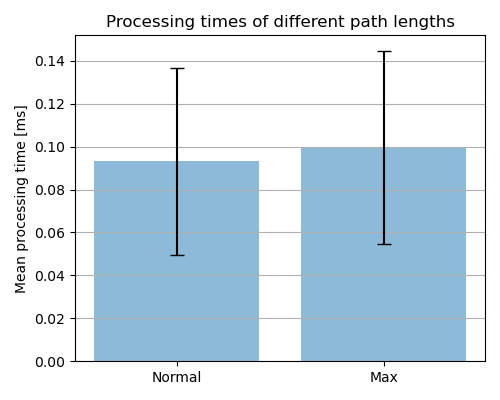
\includegraphics[width=0.75\textwidth]{processing_times_path_lengths.png}
    \caption{Processing times of a SCION ping with different path lengths.}
    \label{fig:path_extension}
\end{figure}

The results indicate that the processing time for the SCION pings with the maximum path length is slightly higher than for the normal SCION pings.
This simple evaluation demonstrates that the impact of extending the path to its maximum length is minimal and largely negligible.


\subsection{Path Header Modification}
This section addresses the modification of the path header by an on-path attacker rather than by the source.
This attack is also discussed in section 7.6.1 of the SCION book \cite{Perrig2022} and works as follows:
An attacker intercepts a SCION packet and modifies the path header by replacing path segments as desired.
The packet is then forwarded along the attacker chosen path rather than the original path inteded by the sender.
These modifications can be reverted by the adversary in replies from the destination (e.g. when the destination inverts the path header to reply), making the sender unaware of the attack.
Our analysis within the CYD SCION network confirmed the feasibility of this attack.

To ensure that the selected path is actually used during transmission, the packet must be integrity protected.
A SCION built in solution would be the SCION packet authenticator option, but this feature is not enabled in the Anapaya routers.
Therefore, clients must implement their own solutions to ensure the integrity of the path header.
For instance, this can be achieved by adding a MAC to the entire packet or by comparing the path information of the received packet with the expected path information.


\subsection{Volumetric Denial of Service}
TODO







\section{Anapaya Router}
This section deals with the security related findings of the Anapaya routers.


\subsection{Secure Shell (SSH)}
The Anapaya routers are accessed via SSH.
All three routers analyzed employ public key authentication and do not allow password authentication.
This is considered a robust security practice, as public key authentication is more secure than password authentication.
This is due to the higher entropy of key compared to passwords, and the fact that keys are not transmitted over the network.
However, our analysis identified some shortcomings with the SSH configuration that could be improved:

\begin{itemize}
    \item Various algorithms use elliptic curves cryptography (ECC) on curves that are believed to have been compromised by the National Security Agency (NSA) \cite{TODO}.
    \item Some MAC algorithms use the broken SHA1 hash function.
    \item The chacha20-poly1305@openssh.com cipher is enabled, which is susceptible to the Terrapin attack (CVE-2023-48795).
    This attack allows message prefix truncation, which enables an attacker to downgrade the security of a connection.
    \item A key exchange algorithm based on Diffie-Hellman group 14 is enabled. It uses a 2048-bit modulus, but only provides 112 bits of security.
    \item Some MAC algorithms are using the encrypt-and-MAC construction, which does not provide integrity of the ciphertext and can possibly leak information of the plaintext.
    It is recommended to use encrypt-then-MAC instead.
    \item Lastly, it should be noted that there are MAC algorithms enabled with a tag length of only 64 bits.
\end{itemize}

To improve the security of the SSH configuration, it is recommended to disable the aforementioned algorithms.
A detailed guide on implementing these changes can be found on this website \cite{sshauditHardeningGuides}.


Furthermore, it was found that the SSH server does not perform any rate limiting on login attempts.
Consequently, it is vulnerable to the DHEat denial of service attack \cite{dheatAttack}, where an attacker sends many Diffie-Hellman keys to the server, which then has to perform numerous expensive modular exponentiation and wasting CPU resources.
An attacker can also just send random big numbers, therefore avoiding computing valid keys.
Our experiments demonstrated that this attack could fully consume the CPU resources of the Anapaya routers in a matter of seconds.
However, due to the SCION dataplane's allocation on a dedicated CPU core, the impact on SCION functionality was minimal.
Nonetheless, other services, such as new SSH login attempts, experienced delays or were not even possible anymore.
To mitigate this attack, it is recommended to implement rate limiting on the SSH server, as it was shown in detail in this blog post \cite{dheatAnalysis}.


\subsection{Ubuntu Compliance}
By attempting to log in to the Anapaya routers via SSH, we observed that there is no banner displayed.
Banners usually contains a legal disclaimer that non-authorized access is prohibited and that activity may be monitored.
This can be crucial for legal compliance and for protecting the organization in the event of unauthorized access.
This is one of a few examples where the Anapaya router does not comply with the Ubuntu security guidelines.
In the following, we will discuss misconfigurations not complying with the CIS Ubuntu Linux 22.04 LTS audit \cite{cisUbuntuLinux2204LTS}.
Numbers in parentheses in this section refer to the corresponding section in the audit.

\begin{itemize}
    \item On two of the three examined routers, there is no password or other re-authentication needed to escalate privileges to root (5.2.4).
    \item While the systems are configured to only accept at least 6 characters long passwords, there is no password policy in place.
    For example, password complexity is not enforced (5.3.3.2.3) and also password reuse is not restricted (5.3.3.3.1).
    \item There is no shell timeout configured, which would log out an inactive user after a certain time (5.4.3.2).
    By setting a timeout, the risk of unauthorized access to the system can be reduced and also frees up resources associated with the idle session.
    \item Shared memory (the directory \texttt{/dev/shm}) can contain executable files, as the noexec option is not set (1.1.2.2.4).
    This option would prevent users from executing binaries from shared memory, which could be used to introduce malicious software into the system.
    \item The directories \texttt{/tmp} as well as \texttt{/var} are not mounted on separate partitions (1.1.2.1.1 and 1.1.2.4.1).
    Both directories are either world-writable or contain world-writable directories or files, which can be exploited to fill up the whole disk and impact the system's availability.
    Additionally, if the directories were mounted on separate partitions with the noexec option, it would prevent other attacks.
    For example an attacker could hard-link a system setuid binary to these locations and wait for it to be updated.
    After such an update, the hard-link would be broken and the attacker has its own copy of the setuid binary.
    If the binary has a security vulnerability it could be exploited to escalate privileges.
    \item There is no separate partition for the \texttt{/home} directory (1.1.2.3.1).
    Again, a user can fill up the disk and impact the system's availability.
    \item The permissions on crontab files are misconfigured (2.4.1.2 - 2.4.1.8) and can be read by unauthorized users.
    These files contain information about scheduled jobs, thus allowing an attacker to gain information about system jobs and potentially exploit them to escalate privileges.
    \item USB storage devices are not restricted (1.1.1.8) and therefore increases the physical attack surface.
    It can be misused to introduce malicious software into the system or to exfiltrate data.
    \item The SSH \texttt{LoginGraceTime} parameter is slightly set too high (5.2.13).
    This parameter specifies the time in seconds that the server allows for a successful login before disconnecting.
    A shorter time would reduce the risk of brute force attacks.
    Currently, the parameter is set to 120 seconds, but it is recommended to set it to 60 seconds.
    \item Root SSH login is enabled (5.2.20).
    By disabling root login over SSH, forces users to authenticate with their own account and then escalate privileges to root.
    This provides a clear audit trail and limits non-repudiation.
\end{itemize}


There are more compliance mismatches found during the audit.
Mostly related to ensure clear audit trails, including monitoring and logging of security-relevant events, or to disable unnecessary kernel modules
The full list of findings can be found \TODO{reference appendix}.

\subsection{Security of systemd Services}
As seen in the previous section, the routers operating system can be optimized to ensure a higher level of security.
In this section, we will focus on the security of the systemd services running on the Anapaya routers.

For this purpose, we analyzed the services by running the \texttt{systemd-analyze security} command.
It evaluates the security settings and provides a score for each systemd service
This score is calculated based on the security features enabled for the service.
A higher score indicates a more exposed and potentially less secure service, whereas it only scores the configuration of the service.

The command can also be run on a single service, which then provides a detailed report on how the score was calculated.
In the following the output of the command and the scoring of the individual services is shown.


\TODO{Maybe try to add emojis here to output}

\begin{lstlisting}[language=bash, deletekeywords={local}, numbers=none, caption={Output of \texttt{systemd-analyze security}}]
$ systemd-analyze security
UNIT                                  EXPOSURE PREDICATE 
ModemManager.service                       6.3 MEDIUM    
appliance-controller.service               9.6 UNSAFE    
appliance-installer.service                9.6 UNSAFE    
apport.service                             9.6 UNSAFE    
caddy.service                              8.8 EXPOSED   
cloud-init-hotplugd.service                9.6 UNSAFE    
containerd.service                         9.6 UNSAFE    
cron.service                               9.6 UNSAFE    
dbus.service                               9.5 UNSAFE    
dm-event.service                           9.5 UNSAFE    
dmesg.service                              9.6 UNSAFE    
docker.service                             9.6 UNSAFE    
emergency.service                          9.5 UNSAFE    
getty@tty1.service                         9.6 UNSAFE    
irqbalance.service                         6.2 MEDIUM    
iscsid.service                             9.5 UNSAFE    
lvm2-lvmpolld.service                      9.5 UNSAFE    
lxd-agent.service                          9.5 UNSAFE    
multipathd.service                         9.5 UNSAFE    
networkd-dispatcher.service                9.6 UNSAFE    
open-vm-tools.service                      9.5 UNSAFE    
packagekit.service                         9.6 UNSAFE    
plymouth-start.service                     9.5 UNSAFE    
polkit.service                             9.6 UNSAFE    
rc-local.service                           9.6 UNSAFE    
rescue.service                             9.5 UNSAFE    
resolvconf.service                         9.5 UNSAFE    
rsyslog.service                            9.6 UNSAFE    
serial-getty@ttyS0.service                 9.6 UNSAFE    
snap.lxd.daemon.service                    9.6 UNSAFE    
snap.lxd.user-daemon.service               9.6 UNSAFE    
snapd.aa-prompt-listener.service           9.6 UNSAFE    
snapd.service                              9.6 UNSAFE    
ssh.service                                9.6 UNSAFE    
systemd-ask-password-console.service       9.4 UNSAFE    
systemd-ask-password-plymouth.service      9.5 UNSAFE    
systemd-ask-password-wall.service          9.4 UNSAFE    
systemd-fsckd.service                      9.5 UNSAFE    
systemd-initctl.service                    9.4 UNSAFE    
systemd-journald.service                   4.3 OK        
systemd-logind.service                     2.8 OK        
systemd-networkd.service                   2.9 OK        
systemd-resolved.service                   2.1 OK        
systemd-rfkill.service                     9.4 UNSAFE    
systemd-timesyncd.service                  2.1 OK        
systemd-udevd.service                      6.9 MEDIUM    
thermald.service                           9.6 UNSAFE    
ubuntu-advantage.service                   9.6 UNSAFE    
udisks2.service                            9.6 UNSAFE    
upower.service                             2.4 OK        
user@1000.service                          9.4 UNSAFE    
uuidd.service                              4.6 OK        
vgauth.service                             9.5 UNSAFE    
\end{lstlisting}

As one can see, many services are considered unsafe.
It is recommended to either disable unused services or to harden the configuration of the services to minimize the attack surface.

For example the \texttt{open-vm-tools} and \texttt{vgauth} services are related to VMware, but as on the routers no virtual machine is being used, these services can be disabled.
Also, the \texttt{ModemManager} service is not needed, as the router is not a modem and does not use mobile broadband (e.g. 2G/3G/4G) connections.
Furthermore, since the routers do not use WiFi or Bluetooth, also the \texttt{systemd-rfkill} service can be disabled.
Ubuntu Advantage is a subscription service that provides additional security features, such as livepatching, compliance checks, technical support and more.
As the Anapaya routers are not connected to the internet and are updated out-of-band, the \texttt{ubuntu-advantage} service is not needed and can be disabled.

Finally, it is also worth taking a closer look if the services can be configured more strictly.
Time did not permit to take a deep dive into the functionality of the services of the \texttt{appliance-controller} and \texttt{appliance-installer} of Anapaya.
However, the high exposure score of 9.6 indicates that these services were not configured to minimize the attack surface.
They enjoy a high level of capabilities and practically no restrictions.
We recommend reviewing the services and to restrict the rights to the minimum required for the services to function properly.


\subsection{Vulnerabilities}


In addition to ensuring the secure configuration of systemd services, it is also crucial to keep the software up-to-date.
This section provides an overview of vulnerabilities identified in the software running on the Anapaya routers.
The vulnerabilities were identified using a Nessus scan and are based on the software version and the Nessus CVE database.

Most identified weaknesses require local access to the system for exploitation.
Vulnerable versions of several software packages were found on the three devices, including \texttt{bash}, \texttt{vim}, \texttt{less}, \texttt{perl}, \texttt{git}, \texttt{tar}, \texttt{Intel Microcode}, \texttt{glibc}, and \texttt{libarchive}.
Some kernel vulnerabilities were also detected, but these require a local privileged attacker (e.g., one with CAP\_NET\_ADMIN capabilities) to exploit them.
The impact of these vulnerabilities ranges from denial of service attacks caused by system crashes to internal information leakage, to privilege escalation.

However, some vulnerabilities were identified that could be exploited remotely.
There are critical vulnerabilities associated with the drivers of the Intel Ethernet controller, which may allow an unauthenticated user to escalate privileges via network access (see CVE-2023-25775 and CVE-2023-45871 for more details).
Although some packages installed on the routers are vulnerable and could be exploited remotely, these packages are not actively used or running on the routers.
It is recommended to either update the affected packages or, preferably, remove unused software entirely to further reduce the attack surface.

A detailed report on all identified vulnerabilities can be found \TODO{reference scan results appropriately}.



\subsection{Docker}
% libc6 libssl1.1 openssl 1.1.1k

The individual services of the Anapaya router are containerized using Docker.
We conducted an automated and manual analysis of these containers to identify potential vulnerabilities.
The Docker images are based on Google's distroless Debian 11.1 base image \cite{githubGitHubGoogleContainerToolsdistroless}.
Such distroless images include only the necessary dependencies and omit a full operating system, which reduces the attack surface and enhances security.
However, our analysis revealed that this base image still contains unused binaries, such as \texttt{openssl}, its corresponding library \texttt{libssl}, and \texttt{c\_rehash}.
Furthermore, these binaries are outdated and vulnerable to various security threats, including command injection, use-after-free, double free, and denial of service attacks.
To improve the security of these Docker containers, it is recommended to remove these unused binaries by switching to the no-ssl variant of the distroless image (see \cite{githubGitHubGoogleContainerToolsdistroless}).

Further analysis of the libraries actually used to run the containers revealed that \texttt{libc} is outdated and has known vulnerabilities.
Although we were unable to directly exploit these vulnerabilities, it is recommended to update \texttt{libc} to the latest version to mitigate potential security threats.
Additionally, using the latest version of the Debian base image (currently version 12) is advisable.

Apart from the base image, it was observed that the live restore feature of Docker is not enabled.
Enabling this feature allows containers to continue running even if the Docker daemon is stopped during a crash or a planned update.
Without this feature, all running containers would stop if the daemon becomes unavailable, potentially leading to data loss and downtime for SCION services.
To ensure a higher availability of the SCION services, it is recommended to enable Docker's live restore feature.

Finally, to further improve availability, we suggest implementing resource limits for the Docker containers.
The inspected systems currently lack resource limits for the Docker containers.
Setting such limits would prevent a single container from consuming all the router's resources, potentially crashing it and impacting all SCION services.



\subsection{Appliance}
Currently, no authentication is required for the CYD SCION users to access the appliance.
Access is granted solely based on knowledge of the IP address of the border router.
This configuration allows users to make significant changes to the border router's configuration, including the following:

\begin{itemize}
    \item Altering firewall rules
    \item Reading and modifying SCION the forwarding key, which is used in the MAC calculations
    \item Changing DNS and NTP server settings
    \item Adding new TRCs
    \item Completely disabling the router
    \item Adding custom authentication options and potentially lock out other users
\end{itemize}

This lack of authentication was also present on the test device, which shows that no default authentication is set up.
This observation is consistent with the official Anapaya documentation, which states that basic authentication is disabled by default \cite{anapayaManagemenDoc}.
To improve the security of the appliance, it is recommended to enable authentication for the appliance.
We also encourage Anapaya to enable basic password authentication by default for newly deployed devices.


\subsection{Web Server}
The appliance is also being served by a web server running on the router, accessible to any AS-local SCION user or any remote user in an AS with a configured SIG connection.
The web server in use is Caddy, version 2.6.4, released in February 2023.
This version is vulnerable to a denial of service attack known as Rapid Reset, which consumes the routers resources and eventually crashes it, thereby taking down all its services, including SCION.
The Rapid Reset attack exploits the HTTP/2 protocol's capability to open multiple streams within a single TCP connection.
An attacker can misuse this feature by simultaneously opening a large number of streams and then instantly closing them again.
By closing the streams right after opening, the attacker ensures that the number of active streams never exceed the limit allowed by the server.
Nonetheless, the server still has to perform substantial work for these canceled requests, including allocating memory for a new stream, parsing the query, performing header decompression, and other tasks \cite{googleWorksNovel}.

By modifying the code in an existing proof-of-concept attack \cite{githubGitHubMicrictorhttp2rststream}, we were able to attack our Anapaya router and finally taking it down withing a few seconds.
Notably, this attack is effective even when the appliance is configured with authentication, as the web server itself is not protected by it.

The recommended solution to mitigate this vulnerability is to update the Caddy web server to version 2.7.5 or later, which addresses the Rapid Reset attack \cite{githubReleasesCaddyservercaddy}.



\subsection{General Recommendations}
% Test device shipped at begging of May 2024:
% - software/system/installed v2.8.0  -> dating back to end of september 2023 (2023-09-27T08:26:15.248888+00:00")
% - appliance v0.34.1                 -> 2023-10-20T13:45:22.216754+00:00

It is crucial to keep the software up-to-date to mitigate potential security threats.
The Anapaya routers should be updated regularly to ensure that the latest security patches are applied.
In May 2024, CYD bought and received a new Anapaya Router.
The system and SCION software version on this new device were outdated and contained the software releases of autumn 2023 (end of September and mid of October).
An improvement on Anapaya's side would be to ship the routers with a more recent software version, ideally the latest release.
\chapter{Discussion}
\label{ch:discussion}

% The discussion is the most difficult part of the thesis to write.
% It should describe wider meaning, importance, and relevance of the thesis and implications for the wider ecosystem.
% In particular, it should answer the following questions:
% * Interpretations: what do the results mean?
%     * Provide a more high-level interpretation of the evaluation results.
% * Implications: why do the results matter?
%     * How does your thesis relate to the related work?
% * Limitations: what can’t the results tell us?
%     * Are there deployment issues and how are they overcome?


In this chapter, we describe the wider meaning and implications of our findings.
It also discusses the limitations of our work and provides recommendations for Anapaya and SCION deployments in general.
% Finally, we outline potential future work that can build on our analysis.


\section{Interpretations and Implications}
The use of a secure MAC algorithm for calculating the $HFAuth$ field in hop fields is crucial as it ensures path integrity and block any path manipulation attacks.
Fortunately, Anapaya employs the same algorithm as the open-source version, facilitating easy verification and reasoning about the security of the system.

However, the absence of DRKey in Anapaya's implementation exposes the system to various attacks, as discussed in \cref{ch:findings}.
Many of these attacks can be mitigated by implementing a custom source authentication mechanism, though this would require a significant effort and likely would not be as lightweight as SPAO based on DRKey.
Other attacks, such as injecting unauthenticated SCMP error message, can only be mitigated with solutions that are supported by each border router in the entire SCION network, such as DRKey which is already provided in SCION.

Due to the proprietary nature of Anapaya's SCION implementation, they can modify certain parts of the protocol, without having to document or justify these changes.
Our analysis revealed a different hop expiry behavior, which leads to the dropping of valid, not-expired SCION packets.
This behavior arguably does not fully comply with the SCION specification and can cause unintended issues in SCION applications that cache and use path information for the full validity period.


Anapaya devices run a recent operating system version with some hardening features enabled.
Nevertheless, additional hardening options can be configured to further enhance the security of the devices.
This includes a hardened SSH configuration, option to limit Docker container resources, patched known vulnerabilities, and improved Ubuntu security compliance.
Many compliance mismatches have already been criticized by Maurer's related work (see \cref{sec:operational-device-security} or his work \cite{Maurer2021}).
Since Maurer's analysis was based on Ubuntu 18.04, his findings could have been used to improve the security standpoint of the current devices running Ubuntu 22.04.
In general, most findings have little impact on SCION or require at least some level of access to the device.
However, the possible Rapid Reset attack on the web server and the lack of authentication on the management system pose significant risks, as they can be exploited without device access.
Fortunately, many issues have been addressed and fixed by Anapaya's latest software releases.
Nonetheless, the absence of default authentication on the management system remains a concern, as it can lead to a severe security compromises.
Specifically, in newer management system versions, it is possible to remove existing SSH keys (thereby locking out legit users) or even to add new SSH keys for the root user.
This lack of authentication can lead to a full device compromise.
To recover from such an attack the device has to be reset and reconfigured entirely, which can lead to a significant downtime.

As demonstrated by our volumetric experiments, protecting the SCION network from volumetric denial-of-service attacks is crucial to maintaining its availability.
Physical separation of SCION and traditional Internet connections ensures that non-SCION adversaries can not disrupt SCION performance through volumetric attacks.

However, the network remains vulnerable to attacks originating within SCION itself.
Our experiments revealed that a malicious SCION adversary could significantly degrade network performance by sending a high volume of SCION packets.
This type of attack can be further intensified by using spoofed source addresses and fake path headers, making the true origin of the attack difficult to trace.

One potential mitigation strategy is the adoption of COLIBRI \cite[Section 10.2]{Perrig2022}, an extension of SCION that enables bandwidth reservation for SCION paths.
However, this approach again relies on the DRKey system to authenticate the source.
An alternative solution available already today is to use hidden paths.
These paths are not publicly advertised and are shared only with trusted parties, such as the CYD Campus network in our case.
Without knowledge of these hidden paths, an attacker would be unable to send SCION packets through them.
It is essential to ensure that the hidden and announced path are physically separated as they share the same underling physical infrastructure.

\section{Limitations}
The analysis of the Anapaya devices was limited to those deployed at CYD Campus.
Other Anapaya customers might have different configurations and security measures in place.
They may also update their devices more frequently and promptly to the latest software versions.
Furthermore, our analysis only covered Anapaya EDGE devices and no CORE or GATE devices.

Due to the time limitations of this thesis, we could not fully analyze the proprietary components of the Anapaya SCION implementation.
Initial reverse engineer efforts did not reveal any critical vulnerabilities.
However, a more comprehensive analysis is necessary to fully understand the security implications of these proprietary changes.

Nevertheless, since all Anapaya customers run the same software, particularly the same SCION implementation, our SCION protocol analysis remains relevant for all Anapaya customers.


\section{Recommendations}

As already emphasized multiple times in the previous chapter and also during discussions with Anapaya, we strongly recommend activating the DRKey feature in their SCION implementation.
Enabling even an experimental version of DRKey would mitigate many attacks and also pave the way for the development of new SCION application that want to employ DRKey.
We further recommend implementing regular key updates to ensure good security hygiene.
Such regular key updates can mitigate the impact of a leaked or compromised key.
Additionally, SCION implementations (both open-source and Anapaya's) should incorporate some sort of outbound filtering to reduce the risk of successful spoofing attacks.

Regarding Anapaya EDGE devices, we recommend adhering to best security practices, such as the CIS benchmarks.
These benchmarks cover various security aspects, such as hardware security, kernel hardening, privilege settings, firewall rules, and more.
Regular security assessments and automated vulnerability scans should be conducted to ensure device security.
It is crucial to address the findings of these assessments by deploying corresponding security updates promptly.
A timely update process is essential to mitigate the risk of successful attacks.

Finally, for a secure SCION deployment, it is essential to ensure that the SCION and traditional Internet connection are physically separated.
This separation minimizes the risk of certain attacks, such as volumetric denial-of-service, from affecting the SCION network and its users.
Additionally, hidden paths should be used to protect the network from volumetric attacks originating from within the SCION network.
These paths should be exclusively shared with trusted parties to prevent unauthorized access and exploitation.
Physical separation of hidden and public SCION paths is a critical measure for maintaining the overall security and resilience of the SCION deployment.


\chapter{Conclusion and Outlook}
\label{ch:conclusion}

% * What have you learnt from the research?
% * What are surprising findings from the work?
% * What future work is possible?
% * Some additional insights.
% * *The conclusion should be very different from the abstract!*


\section{Conclusion}

This thesis set out to critically assess the security of the SCION Internet architecture, with a particular focus on Anapaya's proprietary implementation.
The investigation was driven by the central question:
Can SCION, in its current form as deployed by Anapaya, truly fulfill its promise of a more secure, resilient, and reliable Internet architecture?

To address this question, the thesis conducted a comprehensive analysis across three key areas:

First, an in-depth examination of the deployed Anapaya EDGE devices was performed, revealing several weaknesses.
The study uncovered insecure default configurations, such as inadequate SSH settings and the presence of unused and vulnerable software packages.
More alarmingly, the SCION management system lacked authentication, posing a significant risk of unauthorized access and control over the network infrastructure.
Even with enabled authentication, the management system remained susceptible to attacks capable of crashing the device within seconds and thereby also taking down all SCION services.


The second key area focused on examining the SCION protocol implementation to assess the security of the deployed version and also to identify potential deviations from the open-source version.
The analysis revealed significant flaws, with Anapaya's implementation, including the absence of source authentication within the SCION protocol and the use of persistent master secrets.
These vulnerabilities enable attackers to forge packets, leading to various attack vectors that undermine the integrity and trustworthiness of the network.
Additionally, we observed that SCION packets with nearly expired path information were rejected, highlighting a clear divergence from the SCION protocol specification.

The third and final area of investigation evaluated the impact of volumetric denial-of-service attacks on the SCION infrastructure.
Our experiments demonstrated the importance of physically separating SCION from the traditional Internet to protect against non-SCION adversaries.
Moreover, physical path separation and hidden paths are key to mitigating the impact of volumetric attacks originating within the SCION network.
Otherwise, the network remains vulnerable to such attacks, which can disrupt the availability of SCION services and impact its users.

\\
It became evident that while SCION provides a robust framework, the security of its implementation heavily depends on the rigor of operational practices and the constant evolution of security measures.
The vulnerabilities identified in this thesis highlight the need for continuous security audits, particularly as SCION and its implementations are increasingly deployed in critical infrastructure.

In answering the thesis's key question, this research concludes that while SCION has the potential to fulfill its promise as a next-generation Internet architecture, the current implementation by Anapaya falls short in several critical areas.
The identified weaknesses, if left unaddressed, could undermine the security and reliability that SCION aims to provide.
However, these challenges are not insurmountable.
The findings offer a clear roadmap for improving the security of SCION deployments, emphasizing the need for stronger source authentication mechanisms, more secure device configurations, and the use of hidden paths.

Ultimately, this research contributes to the ongoing development and maturation of SCION, providing valuable insights that can help shape its future evolution.
By addressing the vulnerabilities identified in this thesis, SCION can move closer to realizing its full potential as a secure and resilient Internet architecture for the modern digital world.


\section{Future Work}

While our analysis focused on Anapaya EDGE devices, future research could extend to analyzing Anapaya CORE and GATE devices.
This expansion would help identify differences among the products and uncover potential security issues within them.
Given the rapid development of SCION and Anapaya's products, it would also be beneficial to monitor how the security posture of these devices evolves over time.

Further examination of Anapaya's proprietary SCION components could reveal additional security vulnerabilities.
This could be achieved through reverse engineering of these proprietary elements or by collaborating with Anapaya to gain deeper insights into their implementation.

An in-depth investigation of the SCION control plane presents another promising area for future research.
Control plane issues can significant impact SCION, as it underpins many of its features.
This thesis did not fully cover the control plane in the operational CYD Campus environment due to the associated risks and potential unintended consequences.
Moreover, the control plane is not directly exposed to end users, making it harder for a single end host attacker to exploit.
However, key areas for future work include CP-PKI, certificate management, or path discovery mechanism.

Future research could also explore the development and security of new SCION applications.
This includes how these applications should handle critical scenarios, such as receiving unauthenticated SCMP error messages or managing requests with expired hop fields.

Our work involved volumetric denial-of-service attacks and evaluating its impact on SCION's performance.
It would be interesting to assess the impact of other attacks originating from the traditional Internet.
Additionally, future studies could evaluate the feasibility and the potential effects of these attack when happening directly within the SCION network.

Finally, future studies could investigate SCION traffic sniffing and traffic analysis.
This would help determine what information a passive eavesdropper could collect by intercepting SCION traffic.
Such analysis would be particularly relevant for privacy-sensitive applications that depend on SCION for secure communication.




\bibliographystyle{abbrv}
\bibliography{bibliography, rfc}


\cleardoublepage
\phantomsection{}
\addcontentsline{toc}{chapter}{Declaration of Originality}
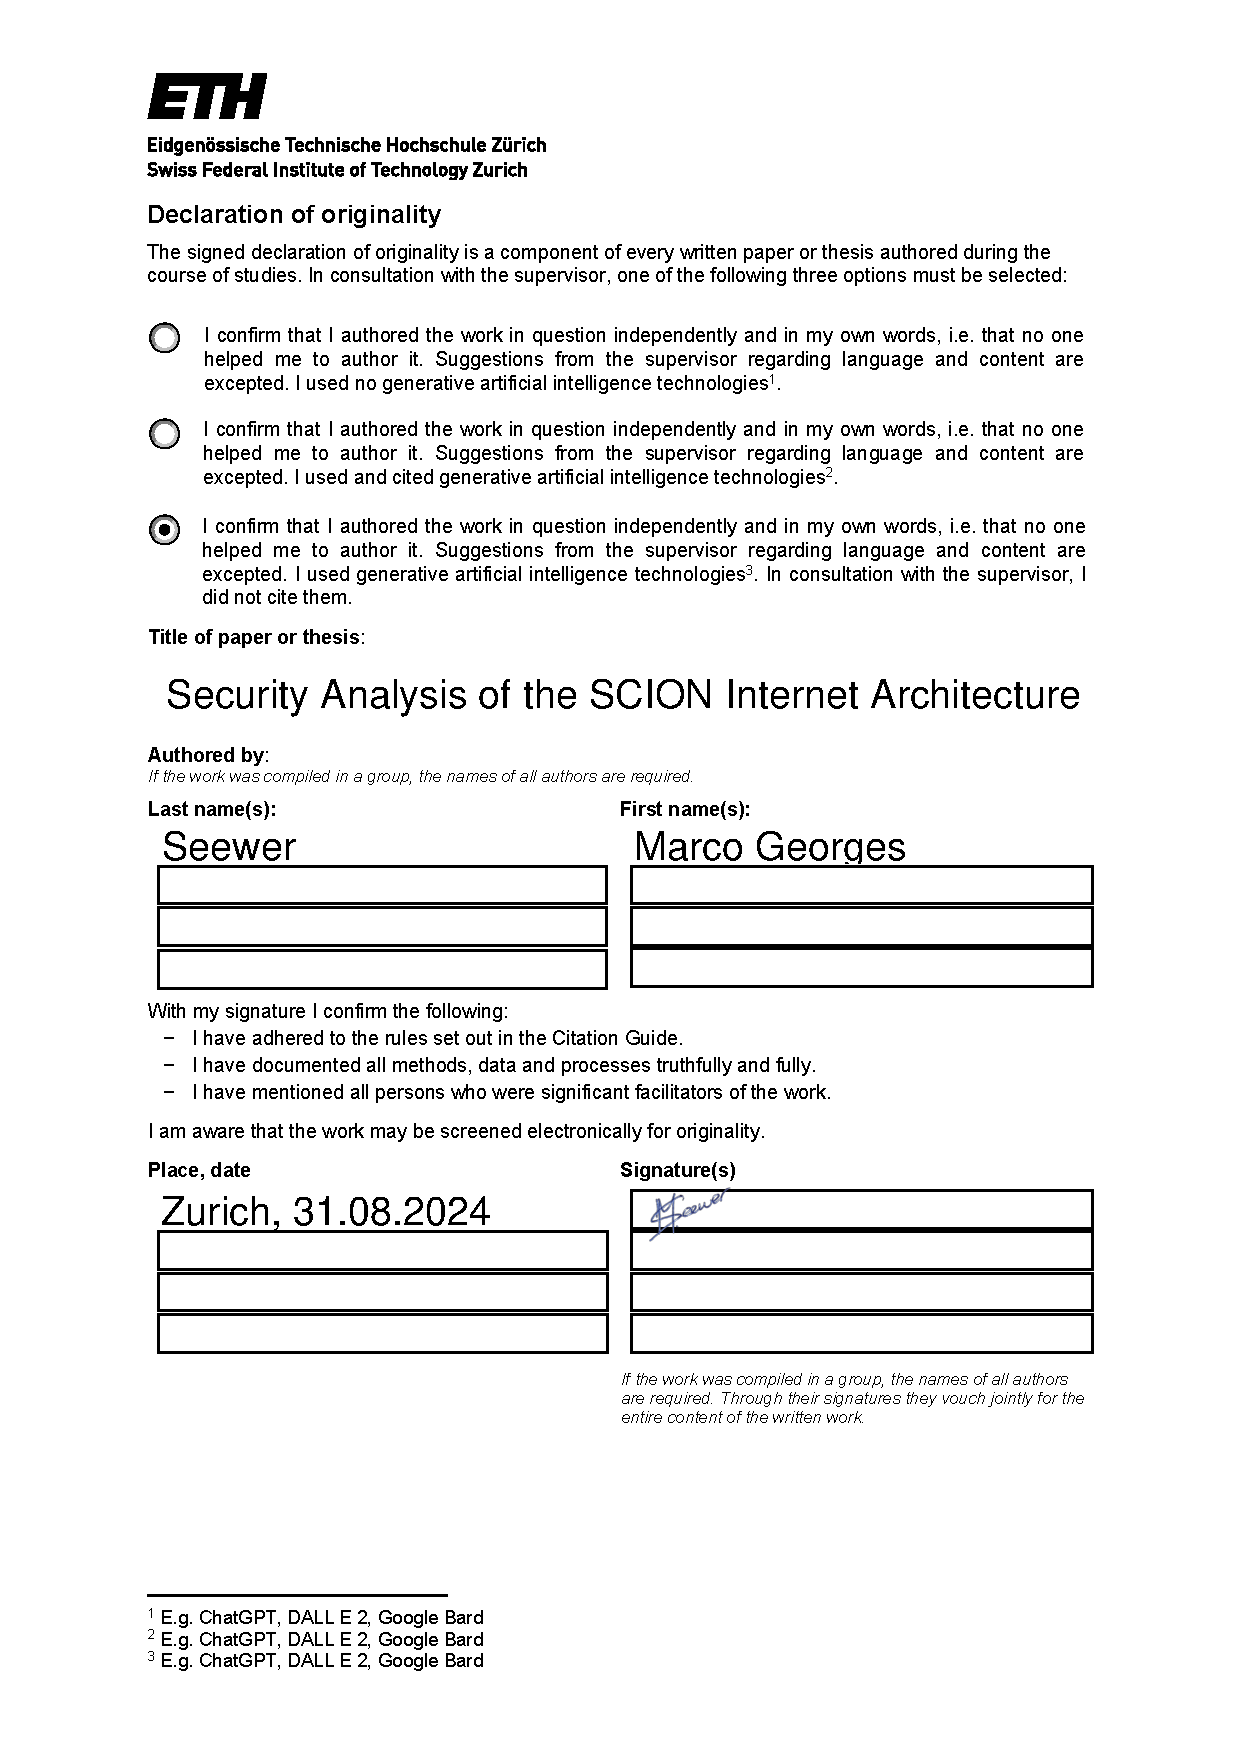
\includepdf[pages={-}]{resources/declaration-originality.pdf} % replace with scan

\end{document}
